\ifx\wholebook\relax \else
% ------------------------

\documentclass{article}
%------------------- Other types of document example ------------------------
%
%\documentclass[twocolumn]{IEEEtran-new}
%\documentclass[12pt,twoside,draft]{IEEEtran}
%\documentstyle[9pt,twocolumn,technote,twoside]{IEEEtran}
%
%-----------------------------------------------------------------------------
%%
% loading packages
%
\newif\ifpdf
\ifx\pdfoutput\undefined % We're not running pdftex
  \pdffalse
\else
  \pdftrue
\fi
%
%
\ifpdf
  \RequirePackage[pdftex,%
            CJKbookmarks,%
       bookmarksnumbered,%
              colorlinks,%
          linkcolor=blue,%
              hyperindex,%
        plainpages=false,%
       pdfstartview=FitH]{hyperref}
\else
  \RequirePackage[dvipdfm,%
             CJKbookmarks,%
        bookmarksnumbered,%
               colorlinks,%
           linkcolor=blue,%
               hyperindex,%
         plainpages=false,%
        pdfstartview=FitH]{hyperref}
  \AtBeginDvi{\special{pdf:tounicode GBK-EUC-UCS2}} % GBK -> Unicode
\fi
\usepackage{hyperref}

% other packages
%-----------------------------------------------------------------------------
\usepackage{graphicx, color}
\usepackage{CJK}
%
% for programming 
%
\usepackage{verbatim}
\usepackage{listings}


\lstdefinelanguage{Smalltalk}{
  morekeywords={self,super,true,false,nil,thisContext}, % This is overkill
  morestring=[d]',
  morecomment=[s]{"}{"},
  alsoletter={\#:},
  escapechar={!},
  literate=
    {BANG}{!}1
    {UNDERSCORE}{\_}1
    {\\st}{Smalltalk}9 % convenience -- in case \st occurs in code
    % {'}{{\textquotesingle}}1 % replaced by upquote=true in \lstset
    {_}{{$\leftarrow$}}1
    {>>>}{{\sep}}1
    {^}{{$\uparrow$}}1
    {~}{{$\sim$}}1
    {-}{{\sf -\hspace{-0.13em}-}}1  % the goal is to make - the same width as +
    %{+}{\raisebox{0.08ex}{+}}1		% and to raise + off the baseline to match -
    {-->}{{\quad$\longrightarrow$\quad}}3
	, % Don't forget the comma at the end!
  tabsize=2
}[keywords,comments,strings]

\lstloadlanguages{C++, Lisp, Smalltalk}

% ======================================================================

\def\BibTeX{{\rm B\kern-.05em{\sc i\kern-.025em b}\kern-.08em
    T\kern-.1667em\lower.7ex\hbox{E}\kern-.125emX}}

\newtheorem{theorem}{Theorem}

%
% mathematics
%
\newcommand{\be}{\begin{equation}}
\newcommand{\ee}{\end{equation}}
\newcommand{\bmat}[1]{\left( \begin{array}{#1} }
\newcommand{\emat}{\end{array} \right) }
\newcommand{\VEC}[1]{\mbox{\boldmath $#1$}}

% numbered equation array
\newcommand{\bea}{\begin{eqnarray}}
\newcommand{\eea}{\end{eqnarray}}

% equation array not numbered
\newcommand{\bean}{\begin{eqnarray*}}
\newcommand{\eean}{\end{eqnarray*}}

\RequirePackage{CJK,CJKnumb,CJKulem,CJKpunct}
% we use CJK as default environment
\AtBeginDocument{\begin{CJK*}{GBK}{song}\CJKtilde\CJKindent\CJKcaption{GB}}
\AtEndDocument{\clearpage\end{CJK*}}

%
% loading packages
%
\newif\ifpdf
\ifx\pdfoutput\undefined % We're not running pdftex
  \pdffalse
\else
  \pdftrue
\fi
%
%
\ifpdf
  \RequirePackage[pdftex,%
       bookmarksnumbered,%
              colorlinks,%
          linkcolor=blue,%
              hyperindex,%
        plainpages=false,%
       pdfstartview=FitH]{hyperref}
\else
  \RequirePackage[dvipdfm,%
        bookmarksnumbered,%
               colorlinks,%
           linkcolor=blue,%
               hyperindex,%
         plainpages=false,%
        pdfstartview=FitH]{hyperref}
\fi
\usepackage{hyperref}

% other packages
%-----------------------------------------------------------------------------
\usepackage{graphicx, color}
%
% for programming 
%
\usepackage{verbatim}
\usepackage{listings}
\usepackage{algorithmic} %for pseudocode
\usepackage{algorithm}


\lstdefinelanguage{Smalltalk}{
  morekeywords={self,super,true,false,nil,thisContext}, % This is overkill
  morestring=[d]',
  morecomment=[s]{"}{"},
  alsoletter={\#:},
  escapechar={!},
  literate=
    {BANG}{!}1
    {UNDERSCORE}{\_}1
    {\\st}{Smalltalk}9 % convenience -- in case \st occurs in code
    % {'}{{\textquotesingle}}1 % replaced by upquote=true in \lstset
    {_}{{$\leftarrow$}}1
    {>>>}{{\sep}}1
    {^}{{$\uparrow$}}1
    {~}{{$\sim$}}1
    {-}{{\sf -\hspace{-0.13em}-}}1  % the goal is to make - the same width as +
    %{+}{\raisebox{0.08ex}{+}}1		% and to raise + off the baseline to match -
    {-->}{{\quad$\longrightarrow$\quad}}3
	, % Don't forget the comma at the end!
  tabsize=2
}[keywords,comments,strings]

\lstloadlanguages{C++, Lisp, Haskell, Python, Smalltalk}

% ======================================================================

\def\BibTeX{{\rm B\kern-.05em{\sc i\kern-.025em b}\kern-.08em
    T\kern-.1667em\lower.7ex\hbox{E}\kern-.125emX}}

\newtheorem{theorem}{Theorem}

%
% mathematics
%
\newcommand{\be}{\begin{equation}}
\newcommand{\ee}{\end{equation}}
\newcommand{\bmat}[1]{\left( \begin{array}{#1} }
\newcommand{\emat}{\end{array} \right) }
\newcommand{\VEC}[1]{\mbox{\boldmath $#1$}}

% numbered equation array
\newcommand{\bea}{\begin{eqnarray}}
\newcommand{\eea}{\end{eqnarray}}

% equation array not numbered
\newcommand{\bean}{\begin{eqnarray*}}
\newcommand{\eean}{\end{eqnarray*}}




\setcounter{page}{1}

\begin{document}

\fi
%--------------------------

% ================================================================
%                 COVER PAGE
% ================================================================

\title{B-Trees}

\author{Larry~LIU~Xinyu
\thanks{{\bfseries Larry LIU Xinyu } \newline
  Email: liuxinyu95@gmail.com \newline}
  }

\markboth{B-Trees}{AlgoXY}

\maketitle

\ifx\wholebook\relax
\chapter{B-Trees}
\numberwithin{Exercise}{chapter}
\section{abstract}
\fi

%{\bfseries Corresponding Author:} Larry LIU Xinyu

% ================================================================
%                 Introduction
% ================================================================
\section{Introduction}
\label{introduction}

B-Tree is important data structure.
It is widely used in modern file systems. Some
are implemented based on B+ tree, which is extended from B-tree.
B-tree is also widely used in database systems.

Some textbooks introduce B-tree with the the problem of how to access a
large block of data on magnetic disks or secondary storage devices\cite{CLRS}.
It is also helpful to understand B-tree as a generalization of balanced binary
search tree\cite{wiki-b-tree}.

Refer to the Figure \ref{fig:btree-example}, It is easy to find the difference
and similarity of B-tree regarding to binary search tree.

\begin{figure}[htbp]
   \begin{center}
	\includegraphics[scale=0.5]{img/btree-example.ps}
   \caption{Example B-Tree} \label{fig:btree-example}
   \end{center}
\end{figure}

Remind the definition of binary search tree. A binary search tree is
\begin{itemize}
\item either an empty node;
\item or a node contains 3 parts, a value, a left child and a right child.
Both children are also binary search trees.
\end{itemize}

The binary search tree satisfies the constraint that.
\begin{itemize}
\item all the values on the left child are not greater than the value of of this node;
\item the value of this node is not greater than any values on the right child.
\end{itemize}

For non-empty binary tree $(L, k, R)$, where $L$, $R$ and $k$
are the left, right children, and the key. Function $Key(T)$ accesses
the key of tree $T$.
The constraint can be represented as the following.

\begin{equation}
\forall x \in L, \forall y \in R \\
\Rightarrow Key(x) \leq k \leq Key(y)
\end{equation}

If we extend this definition to allow multiple keys and children, we get the
B-tree definition.

A B-tree
\begin{itemize}
\item is either empty;
\item or contains $n$ keys, and $n+1$ children, each child is
also a B-Tree, we denote these keys and children as $k_1, k_2, ..., k_n$
and $c_1, c_2, ..., c_n, c_{n+1}$.
\end{itemize}

Figure \ref{fig:btree-node} illustrates a B-Tree node.

\begin{figure}[htbp]
  \centering
	\includegraphics[scale=0.5]{img/btree-node.ps}
  \caption{A B-Tree node} \label{fig:btree-node}
\end{figure}

The keys and children in a node satisfy the following order constraints.

\begin{itemize}
\item Keys are stored in non-decreasing order. that $k_1 \leq k_2 \leq ... \leq k_n$;
\item for each $k_i$, all elements stored in child $c_i$ are not greater
than $k_i$, while $k_i$ is not greater than any values stored in child $c_{i+1}$.
\end{itemize}

The constraints can be represented as in equation (\ref{eq:btree-order})
as well.

\begin{equation}
\forall x_i \in c_i, i=0, 1, ..., n, \Rightarrow x_1 \leq k_1 \leq
x_2 \leq k_2 \leq ... \leq x_n \leq k_n \leq x_{n+1}
\label{eq:btree-order}
\end{equation}

Finally, after adding some constraints to make the tree balanced, we get the
complete B-tree definition.

\begin{itemize}
\item All leaves have the same depth;
\item We define integral number, $t$, as the {\em minimum degree} of
B-tree;
    \begin{itemize}
        \item each node can have at most $2t-1$ keys;
        \item each node can have at least $t-1$ keys, except the root;
    \end{itemize}
\end{itemize}

Consider a B-tree holds $n$ keys. The minimum degree $t \geq 2$.
The height is $h$. All the nodes have at least $t-1$ keys except the
root. The root contains at least 1 key. There are at least 2 nodes
at depth 1, at least $2t$ nodes at depth 2, at least $2t^2$ nodes
at depth 3, ..., finally, there are at least $2t^{h-1}$ nodes at
depth $h$. Times all nodes with $t-1$ except for root,
the total number of keys satisifes the following inequality.

\be
\begin{array}{rl}
n & \geq 1 + (t-1)(2 + 2t + 2t^2 + ... + 2t^{h-1}) \\
  & = 1 + 2(t-1) \displaystyle \sum_{k=0}^{h-1} t^k \\
  & = 1 + 2(t-1) \displaystyle \frac{t^h-1}{t-1} \\
  & = 2t^h - 1
\end{array}
\ee

Thus we have the inequality between the height and the number
of keys.

\be
h \leq \log_t \frac{n+1}{2}
\ee

This is the reason why B-tree is balanced. The simplest B-tree
is so called 2-3-4 tree, where $t=2$, that every node except
root contains 2 or 3 or 4 keys. red-black tree can be mapped
to 2-3-4 tree essentially.

The following Python code shows example B-tree definition.
It explicitly pass $t$ when create a node.

\lstset{language=Python}
\begin{lstlisting}
class BTree:
    def __init__(self, t):
        self.t = t
        self.keys = []
        self.children = []
\end{lstlisting}

B-tree nodes commonly have satellite data as well. We ignore
satellite data for illustration purpose.

In this chapter, we will firstly introduce how to generate B-tree by insertion.
Two different methods will be explained. One is the classic method
as in \cite{CLRS}, that we split the node before insertion if it's full;
the other is the modify-fix approach which is quite similar to the
red-black tree solution \cite{okasaki-rbtree} \cite{wiki-b-tree}.
We will next explain how to delete
key from B-tree and how to look up a key.


% ================================================================
%                 Insertion
% ================================================================
\section{Insertion}
\label{btree-insertion}

B-tree can be created by inserting
keys repeatedly. The basic idea is similar to the binary
search tree. When insert key $x$, from the tree root, we examine all the
keys in the node to find a position where all the keys on the left are
less than $x$, while all the keys on the right are greater than $x$.
If the current node is a leaf node, and it is not full (there are
less then $2t-1$ keys in this node), $x$ will be insert at this position.
Otherwise, the position points to a child node.
We need recursively insert $x$ to it.

\begin{figure}[htbp]
  \centering
  \subfloat[Insert key 22 to the 2-3-4 tree. $22 > 20$, go to the right child; $22 < 26$ go to the first child.]{\includegraphics[scale=0.5]{img/btree-insert-simple1.ps}} \\
  \subfloat[$21 < 22 < 25$, and the leaf isn't full.]{\includegraphics[scale=0.5]{img/btree-insert-simple2.ps}}
  \caption{Insertion is similar to binary search tree.} \label{fig:btree-insert-simple}
\end{figure}

Figure \ref{fig:btree-insert-simple} shows one example. The B-tree illustrated
is 2-3-4 tree. When insert key $x=22$, because it's greater than the root,
the right child contains key 26, 38, 45 is examined next; Since $22 < 26$,
the first child contains key 21 and 25 are examined. This is a leaf
node, and it is not full, key 22 is inserted to this node.

However, if there are $2t-1$ keys in the leaf, the new key $x$ can't
be inserted, because this node is 'full'. When try to insert key 18
to the above example B-tree will meet this problem. There are 2 methods to
solve it.

%=========================================================================
%       Splitting
%=========================================================================
\subsection{Splitting}
\label{split}

If the node is full, one method to solve the problem is to
split to node before insertion.

For a node with $at-1$ keys, it can be divided into 3 parts as shown in
Figure \ref{fig:node-split}. the left part contains the first $t-1$ keys
and $t$ children. The right part contains the rest $t-1$ keys
and $t$ children. Both left part and right part are valid B-tree
nodes. the middle part is the $t$-th key. We can push it up
to the parent node (if the current node is root, then the this key,
with the two children will be the new root).

\begin{figure}[htbp]
  \centering
  \subfloat[Before split]{\includegraphics[scale=0.5]{img/split-node-before.ps}} \\
  \subfloat[After split]{\includegraphics[scale=0.5]{img/split-node-after.ps}}
  \caption{Split node}
  \label{fig:node-split}
\end{figure}

For node $x$, denote $\mathbb{K}(x)$
as keys, $\mathbb{C}(x)$ as children. The $i$-th key as $K_i(x)$, the $j$-th child
as $C_j(x)$. Below algorithm describes how to split the $i$-th child for a given node.

\begin{algorithmic}[1]
\Procedure{Split-Child}{$node, i$}
  \State $x \gets C_i(node)$
  \State $y \gets$ \Call{CREATE-NODE}{}
  \State \Call{Insert}{$\mathbb{K}(node), i, K_t(x)$}
  \State \Call{Insert}{$\mathbb{C}(node), i + 1, y$}
  \State $\mathbb{K}(y) \gets \{K_{t+1}(x), K_{t+2}(x), ..., K_{2t-1}(x)\}$
  \State $\mathbb{K}(x) \gets \{K_1(x), K_2(x), ..., K_{t-1}(x)\}$
  \If{$y$ is not leaf}
    \State $\mathbb{C}(y) \gets \{C_{t+1}(x), C_{t+2}(x), ..., C_{2t}(x)\}$
    \State $\mathbb{C}(x) \gets \{C_1(x), C_2(x), ..., C_t(x)\}$
  \EndIf
\EndProcedure
\end{algorithmic}

The following example Python program implements this child spliting algorithm.

\lstset{language=Python}
\begin{lstlisting}
def split_child(node, i):
    t = node.t
    x = node.children[i]
    y = BTree(t)
    node.keys.insert(i, x.keys[t-1])
    node.children.insert(i+1, y)
    y.keys = x.keys[t:]
    x.keys = x.keys[:t-1]
    if not is_leaf(x):
        y.children = x.children[t:]
        x.children = x.children[:t]
\end{lstlisting}

Where function \texttt{is\_leaf} test if a node is leaf.

\lstset{language=Python}
\begin{lstlisting}
def is_leaf(t):
    return t.children == []
\end{lstlisting}

%=========================================================================
%       Split before insertion
%=========================================================================

After splitting, a key is pushed up to its parent node.
It is quite possible that the parent node has already been full.
And this pushing violates the B-tree property.

In order to solve this problem, we can check from the root along
the path of insertion traversing till the leaf. If there is any node
in this path is full, the splitting is applied. Since the parent
of this node has been examined, it is ensured that there are
less than $2t-1$ keys in the parent. It won't make the
parent full if pushing up one key. This approach only need one single
pass down the tree without any back-tracking.

If the root need splitting, a new node is created as the new root.
There is no keys in this new created root, and the previous root is
set as the only child. After that, splitting is performed top-down.
And we can insert the new key finally.

\begin{algorithmic}[1]
\Function{Insert}{$T, k$}
  \State $r \gets T$
  \If{$r$ is full} \Comment{root is full}
    \State $s \gets$ \Call{CREATE-NODE}{}
    \State $\mathbb{C}(s) \gets \{r\}$
    \State \Call{Split-Child}{$s, 1$}
    \State $r \gets s$
  \EndIf
  \State \Return \Call{Insert-Nonfull}{$r, k$}
\EndFunction
\end{algorithmic}

Where algorithm \textproc{Insert-Nonfull} assumes the node passed in
is not full. If it is a leaf node, the new key is inserted to
the proper position based on the order; Otherwise, the algorithm
finds a proper child node to which the new key will be inserted.
If this child is full, splitting will be performed.

\begin{algorithmic}[1]
\Function{Insert-Nonfull}{$T, k$}
  \If{$T$ is leaf}
    \State $i \gets 1$
    \While{$i \leq |\mathbb{K}(T)| \land k > K_i(T)$}
      \State $i \gets i+1$
    \EndWhile
    \State \Call{Insert}{$\mathbb{K}(T), i, k$}
  \Else
    \State $i \gets |\mathbb{K}(T)|$
    \While{$i>1 \land k < K_i(T)$}
      \State $i \gets i-1$
    \EndWhile
    \If{$C_i(T)$ is full}
      \State \Call{Split-Child}{$T, i$}
      \If{$k > K_i(T)$}
        \State $i \gets i+1$
      \EndIf
    \EndIf
    \State \Call{Insert-Nonfull}{$C_i(T), k$}
  \EndIf
  \State \Return $T$
\EndFunction
\end{algorithmic}

This algorithm is recursive. In B-tree,
the minimum degree $t$ is typically relative to magnetic disk structure.
Even small depth can support huge amount of data
(with $t=10$, maximum to 10 billion data can be stored in a B-tree with height of 10).
The recursion can also be eleminated. This is left as exercise to the reader.

Figure \ref{fig:btree-insert} shows the result of continously inserting
keys G, M, P, X, A, C, D, E, J, K, N, O, R, S, T, U, V, Y, Z to the empty tree.
The first result is the 2-3-4 tree ($t=2$). The second result shows how
it varies when $t=3$.

\begin{figure}[htbp]
  \centering
  \subfloat[2-3-4 tree.]{\includegraphics[scale=0.5]{img/btree-insert-2-3-4.ps}}\\
  \subfloat[$t=3$]{\includegraphics[scale=0.5]{img/btree-insert-3.ps}}
  \caption{Insertion result} \label{fig:btree-insert}
\end{figure}

Below example Python program implements this algorithm.
\lstset{language=Python}
\begin{lstlisting}
def insert(tr, key):
    root = tr
    if is_full(root):
        s = BTree(root.t)
        s.children.insert(0, root)
        split_child(s, 0)
        root = s
    return insert_nonfull(root, key)
\end{lstlisting}

And the insertion to non-full node is implemented as the following.

\begin{lstlisting}
def insert_nonfull(tr, key):
    if is_leaf(tr):
        ordered_insert(tr.keys, key)
    else:
        i = len(tr.keys)
        while i>0 and key < tr.keys[i-1]:
            i = i-1
        if is_full(tr.children[i]):
            split_child(tr, i)
            if key>tr.keys[i]:
                i = i+1
        insert_nonfull(tr.children[i], key)
    return tr
\end{lstlisting}

Where function \texttt{ordered\_insert} is used to insert an element
to an ordered list. Function \texttt{is\_full} tests if a node contains
$2t-1$ keys.

\begin{lstlisting}
def ordered_insert(lst, x):
    i = len(lst)
    lst.append(x)
    while i>0 and lst[i]<lst[i-1]:
        (lst[i-1], lst[i]) = (lst[i], lst[i-1])
        i=i-1

def is_full(node):
    return len(node.keys) >= 2 * node.t - 1
\end{lstlisting}

For the array based collection, append on the tail is much more effective than
insert in other position, because the later takes $O(n)$ time, if the length
of the collection is $n$. The \texttt{ordered_insert} program firstly appends
 the new element at the end of the existing collection, then iterates from the
last element to the first one, and checks if the current two elements next to each other
are ordered. If not, these two elements will be swapped.


\subsubsection{Functional splitting}

For functional algorithm, splitting will return a tuple, which contains the
left part and right as B-Trees, along with a key.

\begin{algorithmic}[1]
\Function{B-TREE-SPLIT}{$node$}
  \State $ks \leftarrow KEYS(node)[1 ... t-1]$
  \State $ks' \leftarrow KEYS(node)[t+1 ... 2t-1]$
  \If{$node$ is not leaf}
    \State $cs \leftarrow CHILDREN(node)[1 ... t]$
    \State $cs' \leftarrow CHILDREN(node)[t ... 2t]$
  \EndIf
  \State \Return $(CREATE-B-TREE(ks, cs), KEYS(node)[t], CREATE-B-TREE(ks', cs'))$
\EndFunction
\end{algorithmic}

\subsubsection*{Split implemented in Haskell}
Haskell prelude provide take/drop functions to get the part
of the list. These functions just returns empty list if the
list passed in is empty. So there is no need to test if
the node is leaf.

\lstset{language=Haskell}
\begin{lstlisting}
split :: BTree a -> (BTree a, a, BTree a)
split (Node ks cs t) = (c1, k, c2) where
    c1 = Node (take (t-1) ks) (take t cs) t
    c2 = Node (drop t ks) (drop t cs) t
    k  = head (drop (t-1) ks)
\end{lstlisting}

When splitting a leaf node, because there is no child at all, the
program simply take the first $t-1$ keys and the last $t-1$ keys
to form two child, and left the $t$-th key as the only key of the
new node. It will return these 3 parts in a list. When splitting
a branch node, children must be also taken into account, that's
why the first $2t-1$ and the last $2t-1$ elements are taken.

% ================================================================
%               Insert and fix method
% ================================================================
\subsection{Insert then fix method}
Another approach to implement B-tree insertion algorithm is just find
the position for the new key and insert it. Since such insertion may
violate B-tree properties. We can then apply a fixing procedure after
that. If a leaf contains too much keys, we split it into 2 leafs and
push a key up to the parent branch node. Of course this operation
may cause the parent node violate the B-tree properties, so the
algorithm need traverse from leaf to root to perform the fixing.

By using recursive implementation these fixing method can also be
realized from top to bottom.

\begin{algorithmic}[1]
\Function{B-TREE-INSERT'}{$T, k$}
  \State \Return $FIX-ROOT(RECURSIVE-INSERT(T, k))$
\EndFunction
\end{algorithmic}

Where $FIX-ROOT$ examine if the root node contains too many keys,
and do splitting if necessary.

\begin{algorithmic}[1]
\Function{FIX-ROOT}{$T$}
  \If{$FULL?(T)$}
    \State $T \leftarrow B-TREE-SPLIT(T)$
  \EndIf
  \State \Return $T$
\EndFunction
\end{algorithmic}

And the inner function $INSERT(T, k)$ will first check if $T$
is leaf node or branch node. It will do directly insertion for leaf
and recursively do insertion for branch.

\begin{algorithmic}[1]
\Function{RECURSIVE-INSERT}{$T, k$}
  \If{$LEAF?(T)$}
    \State $INSERT(KEYS(T), k)$
    \State \Return $T$
  \Else
    \State initialize empty arrays of $k', k'', c', c''$
    \State $i \leftarrow 1$
    \While{$i<=LENGTH(KEYS(T))$ and $KEYS(T)[i]<k$}
      \State $APPEND(k', KEYS(T)[i])$
      \State $APPEND(c', CHILDREN(T)[i])$
      \State $i \leftarrow i+1$
    \EndWhile
    \State $k'' \leftarrow KEYS(T)[i...LENGTH(KEYS(T))]$
    \State $c'' \leftarrow CHILDREN(T)[i+1...LENGTH(CHILDREN(T))]]$
    \State $c \leftarrow CHILDREN(T)[i]$
    \State $left \leftarrow (k', c')$
    \State $right \leftarrow (k'', c'')$
    \State \Return $MAKE-B-TREE(left, RECURSIVE-INSERT(c, k), right)$
  \EndIf
\EndFunction
\end{algorithmic}

Figure \ref{fig:recursive-insert} shows the branch case. The
algorithm first locates the position. for certain key $k_i$,
if the new key $k$ to be inserted satisfy $k_{i-1}<k<k_i$,
Then we need recursively insert $k$ to child $c_i$.

This position divides the node into 3 parts, the left part,
the child $c_i$ and the right part.

\begin{figure}[htbp]
       \begin{center}
       	  \includegraphics[scale=0.5]{img/insert-before.ps}

          a. locate the child to insert,

          \includegraphics[scale=0.5]{img/insert-after.ps}

          b. recursive insert,
        \caption{Insert a key to a branch node} \label{fig:recursive-insert}
       \end{center}
\end{figure}

The procedure $MAKE-B-TREE$ take 3 parameters, which relative to
the left part, the result after insert $k$ to $c_i$ and right part.
It tries to merge these 3 parts into a new B-tree branch node.

However, insert key into a child may make this child violate the
B-tree property if it exceed the limitation of the number of keys
a node can have. $MAKE-B-TREE$ will detect such situation and try
to fix the problem by splitting.

\begin{algorithmic}[1]
\Function{MAKE-B-TREE}{$L, C, R$}
  \If{$FULL?(C)$}
    \State \Return $FIX-FULL(L, C, R)$
  \Else
    \State $T \leftarrow CREATE-NEW-NODE()$
    \State $KEYS(T) \leftarrow KEYS(L) + KEYS(R)$
    \State $CHILDREN(T) \leftarrow CHILDREN(L)+[C]+CHILDREN(R)$
    \State \Return $T$
  \EndIf
\EndFunction
\end{algorithmic}

Where $FIX-FULL$ just calls splitting process.

\begin{algorithmic}[1]
\Function{FIX-FULL}{$L, C, R$}
  \State $(C', K, C'') \leftarrow B-TREE-SPLIT(C)$
  \State $T \leftarrow CREATE-NEW-NODE()$
  \State $KEYS(T) \leftarrow KEYS(L)+[K]+KEYS(R)$
  \State $CHILDREN(T) \leftarrow CHILDREN(L)+[C', C'']+CHILDREN(R)$
  \State \Return $T$
\EndFunction
\end{algorithmic}

Note that splitting may push one extra key up to the parent node.
However, even the push-up causes the violation of B-tree property,
it will be recursively fixed.

\subsubsection*{Insert implemented in Haskell}
Realize the above recursive algorithm in Haskell can implement this
insert-fixing program.

The main program is provided as the following.

\lstset{language=Haskell}
\begin{lstlisting}
insert :: (Ord a)=> BTree a -> a -> BTree a
insert tr x = fixRoot $ ins tr x
\end{lstlisting} %$

It will just call an auxiliary function `ins' then examine and
fix the root node if contains too many keys.

\begin{lstlisting}
import qualified Data.List as L

--...

ins :: (Ord a) => BTree a -> a -> BTree a
ins (Node ks [] t) x = Node (L.insert x ks) [] t
ins (Node ks cs t) x = make (ks', cs') (ins c x) (ks'', cs'')
    where
      (ks', ks'') = L.partition (<x) ks
      (cs', (c:cs'')) = L.splitAt (length ks') cs
\end{lstlisting}

The `ins' function uses pattern matching to handle the two different
cases. If the node to be inserted is leaf, it will call insert
function defined in Haskell standard library, which can insert the
new key $x$ into the proper position to keep the order of the keys.

If the node to be inserted is a branch node, the program will recursively
insert the key to the child which has the range of keys cover $x$.
After that, it will call `make' function to combine the result
together as a new node. the examine and fixing are performed also
by `make' function.

The function `fixRoot' first check if the root node contains too
many keys, if it exceeds the limit, splitting will be applied.
The split result will be used to make a new node, so the total
height of the tree increases.

\begin{lstlisting}
fixRoot :: BTree a -> BTree a
fixRoot (Node [] [tr] _) = tr -- shrink height
fixRoot tr = if full tr then Node [k] [c1, c2] (degree tr)
             else tr
    where
      (c1, k, c2) = split tr
\end{lstlisting}

The following is the implementation of `make' function.

\begin{lstlisting}
make :: ([a], [BTree a]) -> BTree a -> ([a], [BTree a]) -> BTree a
make (ks', cs') c (ks'', cs'')
    | full c = fixFull (ks', cs') c (ks'', cs'')
    | otherwise = Node (ks'++ks'') (cs'++[c]++cs'') (degree c)
\end{lstlisting}

While `fixFull' are given like below.

\begin{lstlisting}
fixFull :: ([a], [BTree a]) -> BTree a -> ([a], [BTree a]) -> BTree a
fixFull (ks', cs') c (ks'', cs'') = Node (ks'++[k]++ks'')
                                         (cs'++[c1,c2]++cs'') (degree c)
    where
      (c1, k, c2) = split c
\end{lstlisting}

In order to print B-tree content out, an auxiliary function `toString'
is provided to convert a B-tree to string.

\begin{lstlisting}
toString :: (Show a)=>BTree a -> String
toString (Node ks [] _) = "("++(L.intercalate ", " (map show ks))++")"
toString tr = "("++(toStr (keys tr) (children tr))++")" where
    toStr (k:ks) (c:cs) = (toString c)++", "++(show k)++", "++(toStr ks cs)
    toStr [] [c] = toString c
\end{lstlisting}

With all the above definition, the insertion program can be verified with
some simple test cases.

\begin{lstlisting}
listToBTree::(Ord a)=>[a]->Int->BTree a
listToBTree lst t = foldl insert (empty t) lst

testInsert = do
  putStrLn $ toString $ listToBTree "GMPXACDEJKNORSTUVYZ" 3
  putStrLn $ toString $ listToBTree "GMPXACDEJKNORSTUVYZ" 2
\end{lstlisting}

Run `testInsert' will generate the following result.

\begin{verbatim}
(('A', 'C', 'D', 'E'), 'G', ('J', 'K'), 'M', ('N', 'O'), 'P', ('R', 'S'),
'T', ('U', 'V', 'X', 'Y', 'Z'))
((('A'), 'C', ('D')), 'E', (('G', 'J', 'K'), 'M', ('N')), 'O', (('P'),
'R', ('S'), 'T', ('U'), 'V', ('X', 'Y', 'Z')))
\end{verbatim}

\begin{figure}[htbp]
  \begin{center}
    \includegraphics[scale=0.5]{img/btree-insert-fp-234.ps}

    a. Insert result of a 2-3-4 tree (insert-fixing method),

    \includegraphics[scale=0.5]{img/btree-insert-fp-3.ps}

    b. Insert result of a B-tree with minimum degree of 3 (insert-fixing method).
    \caption{insert and fixing results} \label{fig:btree-insert-fp}
  \end{center}
\end{figure}

Compare the results output by C++ or Python program with this one,
as shown in figure \ref{fig:btree-insert-fp}
we can found that there are different points. However, the B-tree
built by Haskell program is still valid because all B-tree properties
are satisfied. The main reason for this difference is because of
the approaching change.

\subsubsection*{Insert implemented in Scheme/Lisp}
The main function for insertion in Scheme/Lisp is given as the
following.

\lstset{language=lisp}
\begin{lstlisting}
(define (btree-insert tr x t)
  (define (ins tr x)
    (if (leaf? tr)
	(ordered-insert tr x) ;;leaf
	(let* ((res (partition-by tr x))
	       (left (car res))
	       (c (cadr res))
	       (right (caddr res)))
	  (make-btree left (ins c x) right t))))
  (fix-root (ins tr x) t))
\end{lstlisting}

The program simply calls an internal function and performs fixing
on it. The internal `ins' function examine if the current node
is a leaf node. In case the node is a leaf, it only contains keys,
we can located the position and insert the new key there. Otherwise,
we partition the node into 3 parts, the left part, the child which
the recursive insertion will performed on, and the right part.
The program will do the recursive insertion and then combine
these three part to a new node. fixing will be happened during the
combination.

Function `ordered-insert' can help to traverse a ordered list
and insert the new key to proper position as below.

\begin{lstlisting}
(define (ordered-insert lst x)
  (define (insert-by less-p lst x)
    (if (null? lst)
	(list x)
	(if (less-p x (car lst))
	    (cons x lst)
	    (cons (car lst) (insert-by less-p (cdr lst) x)))))
  (if (string? x)
      (insert-by string<? lst x)
      (insert-by < lst x)))
\end{lstlisting}

In order to deal with B-trees with key types both as string and
as number, we abstract the less-than function as a parameter
and pass it to an internal function.

Function `partition-by' uses a similar approach.

\begin{lstlisting}
(define (partition-by tr x)
  (define (part-by pred tr x)
    (if (= (length tr) 1)
	(list '() (car tr) '())
	(if (pred (cadr tr) x)
	    (let* ((res (part-by pred (cddr tr) x))
		   (left (car res))
		   (c (cadr res))
		   (right (caddr res)))
	      (list (cons-pair (car tr) (cadr tr) left) c right))
	    (list '() (car tr) (cdr tr)))))
  (if (string? x)
      (part-by string<? tr x)
      (part-by < tr x)))
\end{lstlisting}

Where `cons-pair' is a helper function which can put a key, a
child in front of a B-tree.

\begin{lstlisting}
(define (cons-pair c k lst)
  (cons c (cons k lst)))
\end{lstlisting}

In order to fixing the root of a B-tree, which contains too many
keys, a `fix-root' function is provided.

\begin{lstlisting}
(define (full? tr t) ;; t: minimum degree
  (> (length (keys tr))
     (- (* 2 t) 1)))

(define (fix-root tr t)
  (cond ((full? tr t) (split tr t))
	(else tr)))
\end{lstlisting}

When we turn the recursive insertion result to a new node, we
need do fixing if the result node contains too many keys.

\begin{lstlisting}
(define (make-btree l c r t)
  (cond ((full? c t) (fix-full l c r t))
	(else (append l (cons c r)))))

(define (fix-full l c r t)
  (append l (split c t) r))
\end{lstlisting}

With all above facilities, we can test the program for verification.

In order to build the B-tree easily from a list of keys, some simple
helper functions are given.

\begin{lstlisting}
(define (list->btree lst t)
  (fold-left (lambda (tr x) (btree-insert tr x t)) '() lst))

(define (str->slist s)
  (if (string-null? s)
      '()
      (cons (string-head s 1) (str->slist (string-tail s 1)))))
\end{lstlisting}

A same simple test case as the Haskell one is feed to our program.

\begin{lstlisting}
(define (test-insert)
  (list->btree (str->slist "GMPXACDEJKNORSTUVYZBFHIQW") 3))
\end{lstlisting}

Evaluate `test-insert' function can get a B-tree.

\begin{lstlisting}
((("A" "B") "C" ("D" "E" "F") "G" ("H" "I" "J" "K")) "M"
(("N" "O") "P" ("Q" "R" "S") "T" ("U" "V") "W" ("X" "Y" "Z")))
\end{lstlisting}

It is as same as the result output by the Haskell program.

% ================================================================
%               Deletion
% ================================================================
\section{Deletion}

Deletion is another basic operation of B-tree. Delete a key from a
B-tree may cause violating of B-tree balance properties, that a node
can't contains too few keys (no less than $t-1$ keys, where $t$ is
minimum degree).

Similar to the approaches for insertion, we can either do some preparation
so that the node from where the key will be deleted contains enough
keys; or do some fixing after the deletion if the node has too few keys.


% ================================================================
%               Merge before delete method
% ================================================================
\subsection{Merge before delete method}

In textbook\cite{CLRS}, the delete algorithm is given as algorithm description.
The pseudo code is left as exercises. The description can be used
as a good reference when writing the pseudo code.

\subsubsection{Merge before delete algorithm implemented imperatively}

The first case is the trivial, if the key $k$ to be deleted
can be located in node $x$ and $x$ is a leaf node. we can directly
remove $k$ from $x$.

Note that this is a terminal case. For most B-trees which have
not only a leaf node as the root. The program will first examine
non-leaf nodes.

The second case states that, the key $k$ can be located in node $x$,
however, $x$ isn't a leaf node. In this case, there are 3 sub cases.

\begin{itemize}
\item If the child node $y$ precedes $k$ contains enough keys (more than $t$).
We replace $k$ in node $x$ with $k'$, which is
the predecessor of $k$ in child $y$. And recursively remove $k'$
from $y$.

The predecessor of $k$ can be easily located as the last key of child
$y$.

\item If $y$ doesn't contains enough keys, while the child node $z$
follows $k$ contains more than $t$ keys. We replace $k$ in node $x$
with $k''$, which is the successor of $k$ in child $z$. And recursively
remove $k''$ from $z$.

The successor of $k$ can be easily located as the first key of child $z$.

\item Otherwise, if neither $y$, nor $z$ contains enough keys, we
can merge $y$, $k$ and $z$ into one new node, so that this new node
contains $2t-1$ keys. After that, we can then recursively do the removing.

Note that after merge, if the current node doesn't contain any keys,
which means $k$ is the only key in $x$, $y$ and $z$ are the only two
children of $x$. we need shrink the tree height by one.
\end{itemize}

The case 2 is illustrated as in figure \ref{fig:btree-del-case2a},
\ref{fig:btree-del-case2b}, and \ref{fig:btree-del-case2c}.

\begin{figure}[htbp]
  \begin{center}
    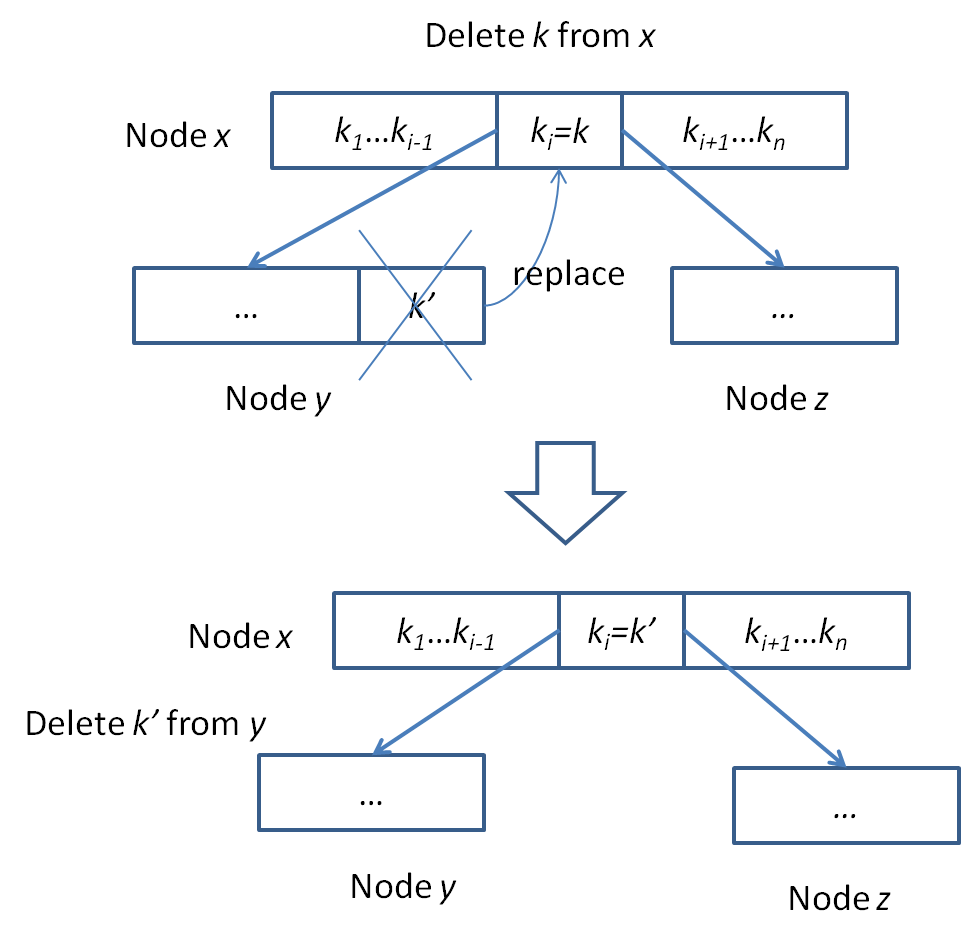
\includegraphics[scale=0.5]{img/btree-del-case2a.eps}
    \caption{case 2a. Replace and delete from predecessor.} \label{fig:btree-del-case2a}
  \end{center}
\end{figure}

\begin{figure}[htbp]
  \begin{center}
    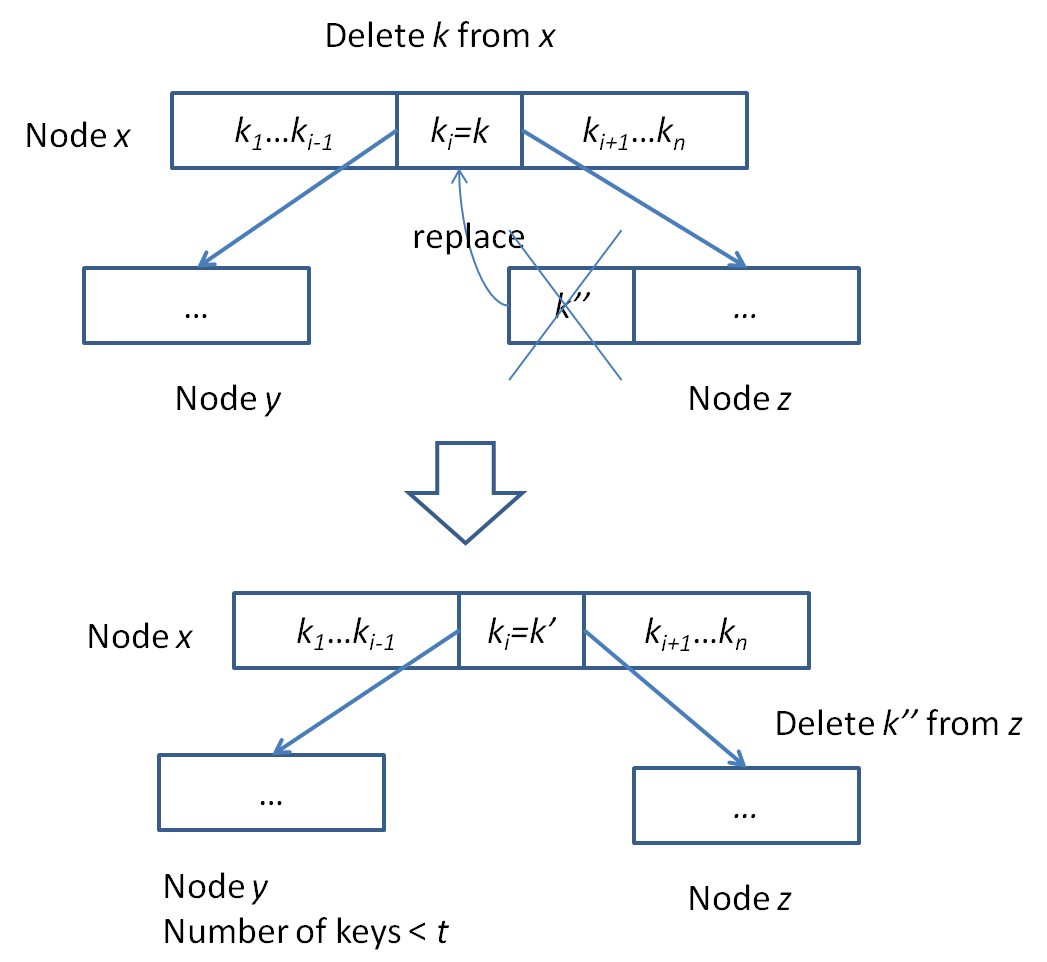
\includegraphics[scale=0.5]{img/btree-del-case2b.eps}
    \caption{case 2b. Replace and delete from successor.} \label{fig:btree-del-case2b}
  \end{center}
\end{figure}

\begin{figure}[htbp]
  \begin{center}
    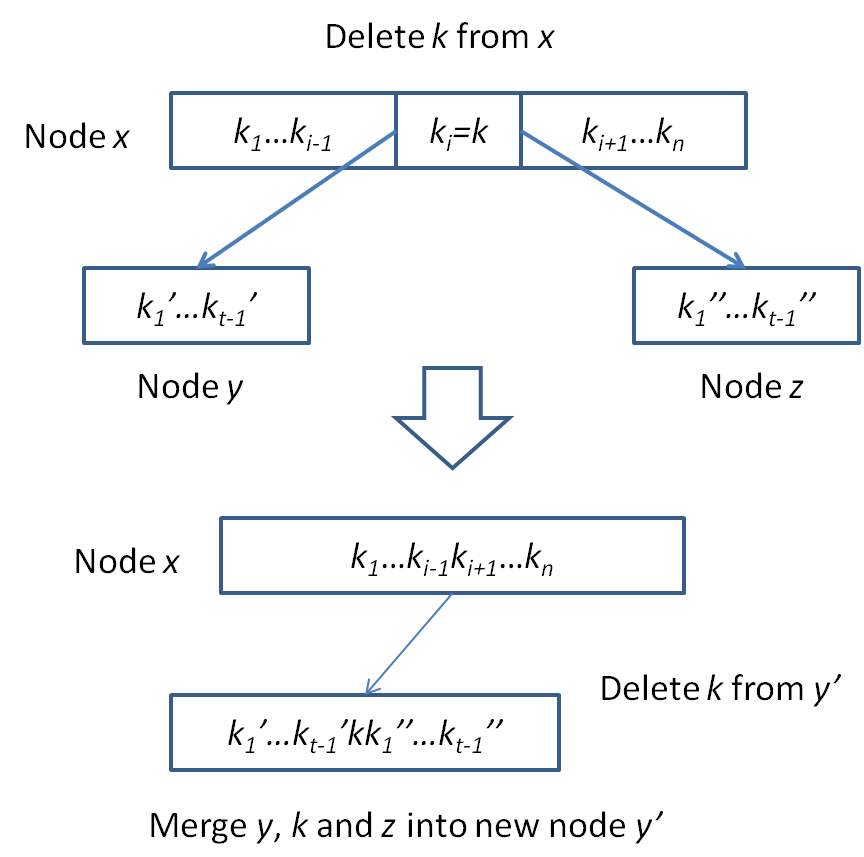
\includegraphics[scale=0.5]{img/btree-del-case2c.eps}
    \caption{case 2c. Merge and delete.} \label{fig:btree-del-case2c}
  \end{center}
\end{figure}

Note that although we use recursive way to delete keys in case 2, the
recursion can be turned into pure imperative way. We'll show such
program in C++ implementation.

the last case states that, if $k$ can't be located in node $x$, the algorithm
need try to find a child node $c_i$ of $x$, so that sub-tree $c_i$ may
contains $k$. Before the deletion is recursively applied in $c_i$, we
need be sure that there are at least $t$ keys in $c_i$. If there are
not enough keys, we need do the following adjustment.

\begin{itemize}
\item We check the two sibling of $c_i$, which are $c_{i-1}$ and $c_{i+1}$.
If either one of them contains enough keys (at least $t$ keys), we move
one key from $x$ down to $c_i$, and move one key from the sibling up to
$x$. Also we need move the relative child from the sibling to $c_i$.

This operation makes $c_i$ contains enough keys OK for deletion. we can
next try to delete $k$ from $c_i$ recursively.

\item In case neither one of the two siblings contains enough keys, we then
merge $c_i$, a key from $x$, and either one of the sibling into a new
node, and do the deletion on this new node.
\end{itemize}

Case 3 is illustrated in figure \ref{fig:btree-del-case3a}, \ref{fig:btree-del-case3b}.

\begin{figure}[htbp]
  \begin{center}
    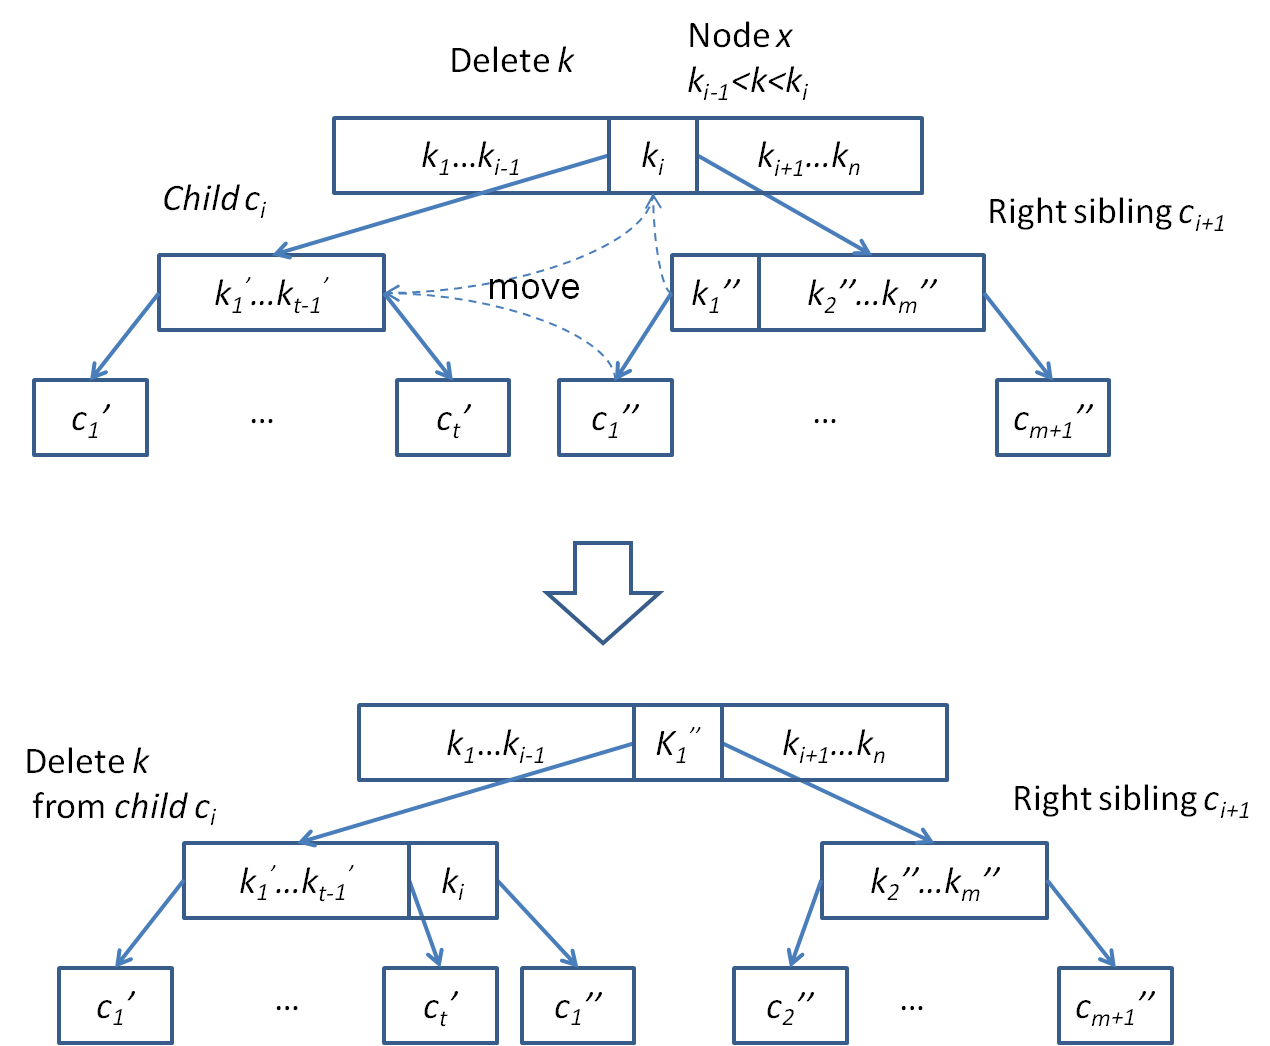
\includegraphics[scale=0.5]{img/btree-del-case3a.eps}
    \caption{case 3a. Borrow from left sibling.} \label{fig:btree-del-case3a}
  \end{center}
\end{figure}

\begin{figure}[htbp]
  \begin{center}
    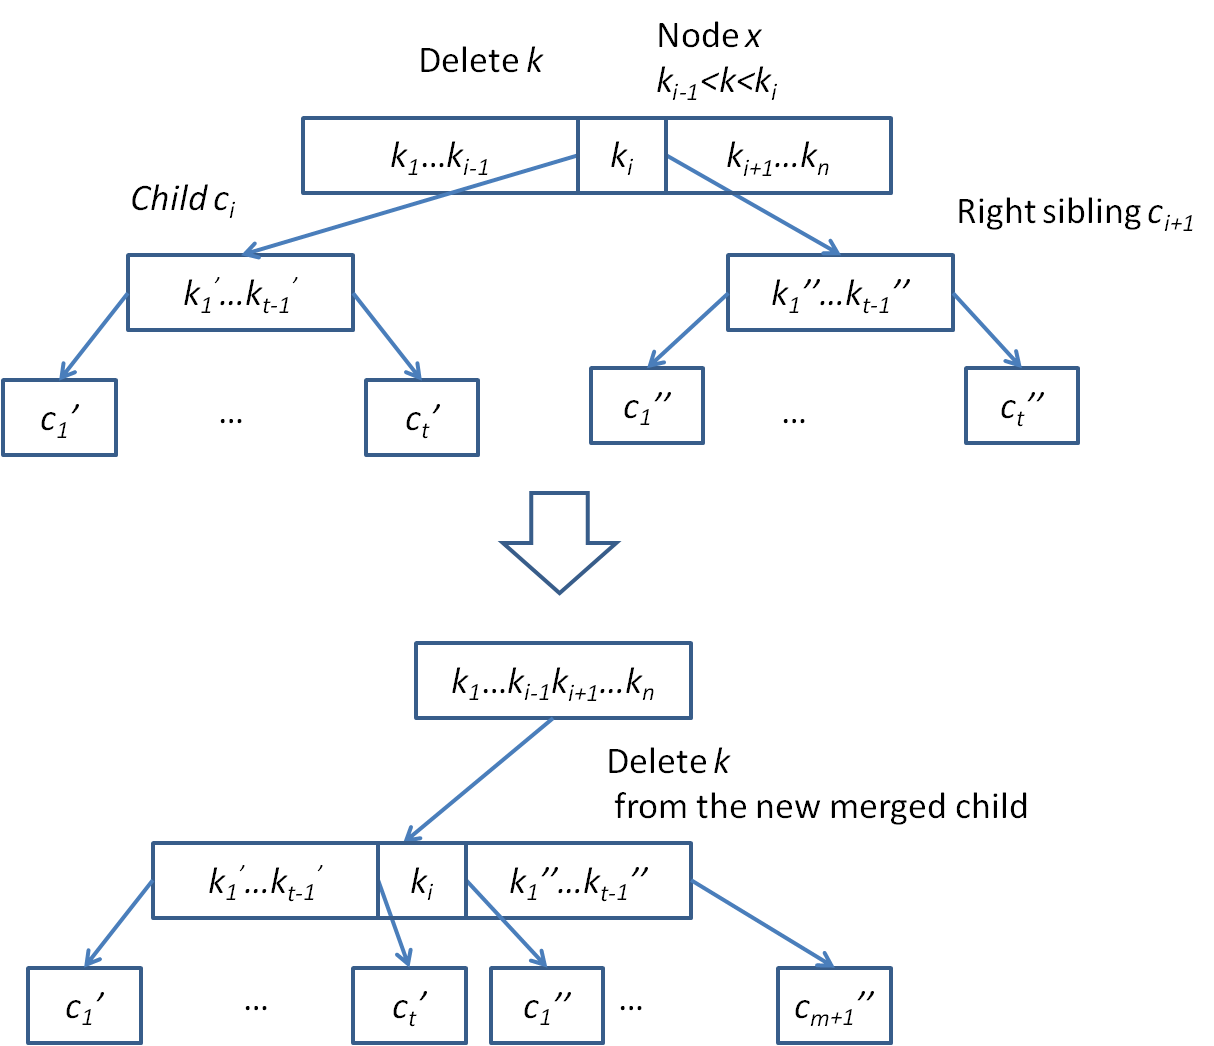
\includegraphics[scale=0.5]{img/btree-del-case3b.eps}
    \caption{case 3b. Borrow Merge and delete.} \label{fig:btree-del-case3b}
  \end{center}
\end{figure}

By implementing the above 3 cases into pseudo code, the B-tree delete algorithm
can be given as the following.

First there are some auxiliary functions to do some simple test and operations
on a B-tree.

\begin{algorithmic}[1]
\Function{CAN-DEL}{$T$}
  \State \Return number of keys of  $T \ge t$
\EndFunction
\end{algorithmic}

Function $CAN-DEL$ test if a B-tree node contains enough keys (no less than
$t$ keys).

\begin{algorithmic}[1]
\Procedure{MERGE-CHILDREN}{$T, i$} \Comment{Merge children $i$ and $i+1$}
  \State $x \leftarrow CHILDREN(T)[i]$
  \State $y \leftarrow CHILDREN(T)[i+1]$
  \State $APPEND(KEYS(x), KEYS(T)[i])$
  \State $CONCAT(KEYS(x), KEYS(y))$
  \State $CONCAT(CHILDREN(x), CHILDREN(y)$
  \State $REMOVE(KEYS(T), i)$
  \State $REMOVE(CHILDREN(T), i+1)$
\EndProcedure
\end{algorithmic}

Procedure $MERGE-CHILDREN$ merges the $i$-th child, the $i$-th key,
and $i+1$-th child of node $T$ into a new child, and remove the
$i$-th key and $i+1$-th child after merging.

With these helper functions, the main algorithm of B-tree deletion is described
as below.

\begin{algorithmic}[1]
\Function{B-TREE-DELETE}{$T, k$}
  \State $i \leftarrow 1$
  \While{$i <= LENGTH(KEYS(T))$}
    \If{$k = KEYS(T)[i]$}
      \If{$T$ is leaf} \Comment{case 1}
        \State $REMOVE(KEYS(T), k)$
      \Else \Comment{case 2}
        \If{$CAN-DEL(CHILDREN(T)[i])$} \Comment{case 2a}
          \State $KEYS(T)[i] \leftarrow LAST-KEY(CHILDREN(T)[i])$
          \State $B-TREE-DELETE(CHILDREN(T)[i], KEYS(T)[i])$
        \ElsIf{$CAN-DEL(CHILDREN(T)[i+1])$} \Comment{case 2b}
          \State $KEYS(T)[i] \leftarrow FIRST-KEY(CHILDREN(T)[i+1])$
          \State $B-TREE-DELETE(CHILDREN(T)[i+1], KEYS(T)[i])$
        \Else \Comment{case 2c}
          \State $MERGE-CHILDREN(T, i)$
          \State $B-TREE-DELETE(CHILDREN(T)[i], k)$
          \If{$KEYS(T) = NIL$}
            \State $T \leftarrow CHILDREN(T)[i]$ \Comment{Shrinks height}
          \EndIf
        \EndIf
      \EndIf
      \State \Return $T$
    \ElsIf{$k < KEYS(T)[i]$}
      \State $BREAK$
    \Else
      \State $i \leftarrow i+1$
    \EndIf
  \EndWhile
  \Statex
  \If{$T$ is leaf}
    \State \Return $T$ \Comment{$k$ doesn't exist in $T$ at all}
  \EndIf
  \If{not $CAN-DEL(CHILDREN(T)[i])$}  \Comment{case 3}
    \If{$i>1$ and $CAN-DEL(CHILDREN(T)[i-1])$} \Comment{case 3a: left sibling}
      \State $INSERT(KEYS(CHILDREN(T)[i]), KEYS(T)[i-1])$
      \State $KEYS(T)[i-1] \leftarrow POP-BACK(KEYS(CHILDREN(T)[i-1]))$
      \If{$CHILDREN(T)[i]$ isn't leaf}
        \State $c \leftarrow POP-BACK(CHILDREN(CHILDREN(T)[i-1]))$
        \State $INSERT(CHILDREN(CHILDREN(T)[i]), c)$
      \EndIf
    \ElsIf{$i<=LENGTH(CHILDREN(T))$ and $CAN-DEL(CHILDREN(T)[i+1]$} \Comment{case 3a: right sibling}
      \State $APPEND(KEYS(CHILDREN(T)[i]), KEYS(T)[i])$
      \State $KEYS(T)[i] \leftarrow POP-FRONT(KEYS(CHILDREN(T)[i+1]))$
      \If{$CHILDREN(T)[i]$ isn't leaf}
        \State $c \leftarrow POP-FRONT(CHILDREN(CHILDREN(T)[i+1]))$
        \State $APPEND(CHILDREN(CHILDREN(T)[i]), c)$
      \EndIf
    \Else \Comment{case 3b}
      \If{$i>1$}
        \State $MERGE-CHILDREN(T, i-1)$
      \Else
        \State $MERGE-CHILDREN(T, i)$
      \EndIf
    \EndIf
  \EndIf
  \State $B-TREE-DELETE(CHILDREN(T)[i], k)$ \Comment {recursive delete}
  \If{$KEYS(T) = NIL$} \Comment {Shrinks height}
    \State $T \gets CHILDREN(T)[1]$
  \EndIf
  \State \Return $T$
\EndFunction
\end{algorithmic}

\subsubsection{Merge before deletion algorithm implemented in C++}
The C++ implementation given here isn't simply translate the above
pseudo code into C++. The recursion can be eliminated in a pure
imperative program.

In order to simplify some B-tree node operation, some auxiliary
member functions are added to the B-tree node class definition.

\lstset{language=C++}
\begin{lstlisting}
template<class K, int t>
struct BTree{
  //...
  // merge children[i], keys[i], and children[i+1] to one node
  void merge_children(int i){
    BTree<K, t>* x = children[i];
    BTree<K, t>* y = children[i+1];
    x->keys.push_back(keys[i]);
    concat(x->keys, y->keys);
    concat(x->children, y->children);
    keys.erase(keys.begin()+i);
    children.erase(children.begin()+i+1);
    y->children.clear();
    delete y;
  }

  key_type replace_key(int i, key_type key){
    keys[i]=key;
    return key;
  }

  bool can_remove(){ return keys.size() >=t; }
  //...
\end{lstlisting}

Function `replace\_key' can update the $i$-th key of a node with a
new value. Typically, this new value is pulled from a child node as
described in deletion algorithm. It will return the new value.

Function `can\_remove' will test if a node contains enough keys for
further deletion.

Function `merge\_children' can merge the $i$-th child, the $i$-th key,
and the $i+1$-th children into one node. This operation is reverse
operation of splitting, it can double the keys of a node, so that
such adjustment can ensure a node has enough keys for further deleting.

Note that, unlike the other languages equipped with GC, in C++ program,
the memory must be released after merging.

This function uses `concat' function to concatenate two collections.
It is defined as the following.

\begin{lstlisting}
template<class Coll>
void concat(Coll& x, Coll& y){
  std::copy(y.begin(), y.end(),
            std::insert_iterator<Coll>(x, x.end()));
}
\end{lstlisting}

With these helper functions, the main program of B-tree deleting
is given as below.

\begin{lstlisting}
template<class T>
T* del(T* tr, typename T::key_type key){
  T* root(tr);
  while(!tr->leaf()){
    unsigned int i = 0;
    bool located(false);
    while(i < tr->keys.size()){
      if(key == tr->keys[i]){
        located = true;
        if(tr->children[i]->can_remove()){ //case 2a
          key = tr->replace_key(i, tr->children[i]->keys.back());
          tr->children[i]->keys.pop_back();
          tr = tr->children[i];
        }
        else if(tr->children[i+1]->can_remove()){ //case 2b
          key = tr->replace_key(i, tr->children[i+1]->keys.front());
          tr->children[i+1]->keys.erase(tr->children[i+1]->keys.begin());
          tr = tr->children[i+1];
        }
        else{ //case 2c
          tr->merge_children(i);
          if(tr->keys.empty()){ //shrinks height
            T* temp = tr->children[0];
            tr->children.clear();
            delete tr;
            tr = temp;
          }
        }
        break;
      }
      else if(key > tr->keys[i])
        i++;
      else
        break;
    }
    if(located)
      continue;
    if(!tr->children[i]->can_remove()){ //case 3
      if(i>0 && tr->children[i-1]->can_remove()){
        // case 3a: left sibling
        tr->children[i]->keys.insert(tr->children[i]->keys.begin(),
                                     tr->keys[i-1]);
        tr->keys[i-1] = tr->children[i-1]->keys.back();
        tr->children[i-1]->keys.pop_back();
        if(!tr->children[i]->leaf()){
          tr->children[i]->children.insert(tr->children[i]->children.begin(),
                                           tr->children[i-1]->children.back());
          tr->children[i-1]->children.pop_back();
        }
      }
      else if(i<tr->children.size() && tr->children[i+1]->can_remove()){
        // case 3a: right sibling
        tr->children[i]->keys.push_back(tr->keys[i]);
        tr->keys[i] = tr->children[i+1]->keys.front();
        tr->children[i+1]->keys.erase(tr->children[i+1]->keys.begin());
        if(!tr->children[i]->leaf()){
          tr->children[i]->children.push_back(tr->children[i+1]->children.front());
          tr->children[i+1]->children.erase(tr->children[i+1]->children.begin());
        }
      }
      else{
        if(i>0)
          tr->merge_children(i-1);
        else
          tr->merge_children(i);
      }
    }
    tr = tr->children[i];
  }
  tr->keys.erase(remove(tr->keys.begin(), tr->keys.end(), key),
                 tr->keys.end());
  if(root->keys.empty()){ //shrinks height
    T* temp = root->children[0];
    root->children.clear();
    delete root;
    root = temp;
  }
  return root;
}
\end{lstlisting}

Please note how the recursion be eliminated. The main loop terminates
only if the current node which is examined is a leaf. Otherwise, the
program will go through the B-tree along the path which may contains
the key to be deleted, and do proper adjustment including borrowing
keys from other nodes, or merging to make the candidate nodes along
this path all have enough keys to perform deleting.

In order to verify this program, a quick and simple parsing function
which can turn a B-tree description string into a B-tree is provided.
Error handling of parsing is omitted for illusion purpose.

\begin{lstlisting}
template<class T>
T* parse(std::string::iterator& first, std::string::iterator last){
  T* tr = new T;
  ++first; //'('
  while(first!=last){
    if(*first=='('){ //child
      tr->children.push_back(parse<T>(first, last));
    }
    else if(*first == ',' || *first == ' ')
      ++first; //skip deliminator
    else if(*first == ')'){
      ++first;
      return tr;
    }
    else{ //key
      typename T::key_type key;
      while(*first!=',' && *first!=')')
        key+=*first++;
      tr->keys.push_back(key);
    }
  }
  //should never run here
  return 0;
}

template<class T>
T* str_to_btree(std::string s){
  std::string::iterator first(s.begin());
  return parse<T>(first, s.end());
}
\end{lstlisting}

After that, the testing can be performed as below.

\begin{lstlisting}
  void test_delete(){
    std::cout<<"test delete...\n";
    const char* s="(((A, B), C, (D, E, F), G, (J, K, L), M, (N, O)), "
                  "P, ((Q, R, S), T, (U, V), X, (Y, Z)))";
    typedef BTree<std::string, 3> BTr;
    BTr* tr = str_to_btree<BTr>(s);
    std::cout<<"before delete:\n"<<btree_to_str(tr)<<"\n";
    const char* ks[] = {"F", "M", "G", "D", "B", "U"};
    for(unsigned int i=0; i<sizeof(ks)/sizeof(char*); ++i)
      tr=__test_del__(tr, ks[i]);
    delete tr;
  }

  template<class T>
  T* __test_del__(T* tr, typename T::key_type key){
    std::cout<<"delete "<<key<<"==>\n";
    tr = del(tr, key);
    std::cout<<btree_to_str(tr)<<"\n";
    return tr;
  }
\end{lstlisting}

Run `test\_delete' will generate the below result.

\begin{verbatim}
test delete...
before delete:
(((A, B), C, (D, E, F), G, (J, K, L), M, (N, O)), P, ((Q, R, S), T, (U, V), X, (Y, Z)))
delete F==>
(((A, B), C, (D, E), G, (J, K, L), M, (N, O)), P, ((Q, R, S), T, (U, V), X, (Y, Z)))
delete M==>
(((A, B), C, (D, E), G, (J, K), L, (N, O)), P, ((Q, R, S), T, (U, V), X, (Y, Z)))
delete G==>
(((A, B), C, (D, E, J, K), L, (N, O)), P, ((Q, R, S), T, (U, V), X, (Y, Z)))
delete D==>
((A, B), C, (E, J, K), L, (N, O), P, (Q, R, S), T, (U, V), X, (Y, Z))
delete B==>
((A, C), E, (J, K), L, (N, O), P, (Q, R, S), T, (U, V), X, (Y, Z))
delete U==>
((A, C), E, (J, K), L, (N, O), P, (Q, R), S, (T, V), X, (Y, Z))
\end{verbatim}

Figure \ref{fig:result-del1}, \ref{fig:result-del2}, and \ref{fig:result-del3}
show this deleting test process step by step. The nodes modified are shaded.
The first 5 steps are as same as the example shown in textbook\cite{CLRS} figure 18.8.

\begin{figure}[htbp]
    \begin{center}
      \includegraphics[scale=0.5]{img/btree-del-before.ps}

      a. A B-tree before performing deleting;

      \includegraphics[scale=0.5]{img/btree-del-F.ps}

      b. After delete key 'F', case 1;
      \caption{Result of B-tree deleting program (1)} \label{fig:result-del1}
    \end{center}
\end{figure}

\begin{figure}[htbp]
    \begin{center}
      \includegraphics[scale=0.5]{img/btree-del-M.ps}

      c. After delete key 'M', case 2a;

      \includegraphics[scale=0.5]{img/btree-del-G.ps}

      d. After delete key 'G', case 2c;
      \caption{Result of B-tree deleting program (2)} \label{fig:result-del2}
    \end{center}
\end{figure}

\begin{figure}[htbp]
    \begin{center}
      \includegraphics[scale=0.5]{img/btree-del-D.ps}

      e. After delete key 'D', case 3b, and height is shrunk;

      \includegraphics[scale=0.5]{img/btree-del-B.ps}

      f. After delete key 'B', case 3a, borrow from right sibling;

      \includegraphics[scale=0.5]{img/btree-del-U.ps}

      g. After delete key 'U', case 3a, borrow from left sibling;

      \caption{Result of B-tree deleting program (3)} \label{fig:result-del3}
    \end{center}
\end{figure}


\subsubsection{Merge before deletion algorithm implemented in Python}
In Python implementation, detailed memory management can be handled by
GC. Similar as the C++ program, some auxiliary member functions
are added to B-tree node definition.

\lstset{language=Python}
\begin{lstlisting}
class BTreeNode:
    #...
    def merge_children(self, i):
        #merge children[i] and children[i+1] by pushing keys[i] down
        self.children[i].keys += [self.keys[i]]+self.children[i+1].keys
        self.children[i].children += self.children[i+1].children
        self.keys.pop(i)
        self.children.pop(i+1)

    def replace_key(self, i, key):
        self.keys[i] = key
        return key

    def can_remove(self):
        return len(self.keys) >= self.t
\end{lstlisting}

The member function names are same with the C++ program, so that the
meaning for each of them can be referred in previous sub section.

In contrast to the C++ program, a recursion approach similar to the
pseudo code is used in this Python program.

\begin{lstlisting}
def B_tree_delete(tr, key):
    i = len(tr.keys)
    while i>0:
        if key == tr.keys[i-1]:
            if tr.leaf:  # case 1 in CLRS
                tr.keys.remove(key)
                #disk_write(tr)
            else: # case 2 in CLRS
                if tr.children[i-1].can_remove(): # case 2a
                    key = tr.replace_key(i-1, tr.children[i-1].keys[-1])
                    B_tree_delete(tr.children[i-1], key)
                elif tr.children[i].can_remove(): # case 2b
                    key = tr.replace_key(i-1, tr.children[i].keys[0])
                    B_tree_delete(tr.children[i], key)
                else: # case 2c
                    tr.merge_children(i-1)
                    B_tree_delete(tr.children[i-1], key)
                    if tr.keys==[]: # tree shrinks in height
                        tr = tr.children[i-1]
            return tr
        elif key > tr.keys[i-1]:
            break
        else:
            i = i-1
    # case 3
    if tr.leaf:
        return tr #key doesn't exist at all
    if not tr.children[i].can_remove():
        if i>0 and tr.children[i-1].can_remove(): #left sibling
            tr.children[i].keys.insert(0, tr.keys[i-1])
            tr.keys[i-1] = tr.children[i-1].keys.pop()
            if not tr.children[i].leaf:
                tr.children[i].children.insert(0, tr.children[i-1].children.pop())
        elif i<len(tr.children) and tr.children[i+1].can_remove(): #right sibling
            tr.children[i].keys.append(tr.keys[i])
            tr.keys[i]=tr.children[i+1].keys.pop(0)
            if not tr.children[i].leaf:
                tr.children[i].children.append(tr.children[i+1].children.pop(0))
        else: # case 3b
            if i>0:
                tr.merge_children(i-1)
            else:
                tr.merge_children(i)
    B_tree_delete(tr.children[i], key)
    if tr.keys==[]: # tree shrinks in height
        tr = tr.children[0]
    return tr
\end{lstlisting}

In order to verify the deletion program, similar test cases are
fed to the function.

\begin{lstlisting}
def test_delete():
    print "test delete"
    t = 3
    tr = BTreeNode(t, False)
    tr.keys=["P"]
    tr.children=[BTreeNode(t, False), BTreeNode(t, False)]
    tr.children[0].keys=["C", "G", "M"]
    tr.children[0].children=[BTreeNode(t), BTreeNode(t), BTreeNode(t), BTreeNode(t)]
    tr.children[0].children[0].keys=["A", "B"]
    tr.children[0].children[1].keys=["D", "E", "F"]
    tr.children[0].children[2].keys=["J", "K", "L"]
    tr.children[0].children[3].keys=["N", "O"]
    tr.children[1].keys=["T", "X"]
    tr.children[1].children=[BTreeNode(t), BTreeNode(t), BTreeNode(t)]
    tr.children[1].children[0].keys=["Q", "R", "S"]
    tr.children[1].children[1].keys=["U", "V"]
    tr.children[1].children[2].keys=["Y", "Z"]
    print B_tree_to_str(tr)
    lst = ["F", "M", "G", "D", "B", "U"]
    reduce(__test_del__, lst, tr)

def __test_del__(tr, key):
    print "delete", key
    tr = B_tree_delete(tr, key)
    print B_tree_to_str(tr)
    return tr
\end{lstlisting}

In this test case, the B-tree is constructed manually. It is identical to
the B-tree built in C++ deleting test case. Run the test function will
generate the following result.

\begin{verbatim}
test delete
(((A, B), C, (D, E, F), G, (J, K, L), M, (N, O)), P, ((Q, R, S), T, (U, V), X, (Y, Z)))
delete F
(((A, B), C, (D, E), G, (J, K, L), M, (N, O)), P, ((Q, R, S), T, (U, V), X, (Y, Z)))
delete M
(((A, B), C, (D, E), G, (J, K), L, (N, O)), P, ((Q, R, S), T, (U, V), X, (Y, Z)))
delete G
(((A, B), C, (D, E, J, K), L, (N, O)), P, ((Q, R, S), T, (U, V), X, (Y, Z)))
delete D
((A, B), C, (E, J, K), L, (N, O), P, (Q, R, S), T, (U, V), X, (Y, Z))
delete B
((A, C), E, (J, K), L, (N, O), P, (Q, R, S), T, (U, V), X, (Y, Z))
delete U
((A, C), E, (J, K), L, (N, O), P, (Q, R), S, (T, V), X, (Y, Z))
\end{verbatim}

This result is as same as the one output by C++ program.

% ================================================================
%               Delete and fix method
% ================================================================

\subsection{Delete and fix method}

From previous sub-sections, we see how complex is the deletion algorithm,
There are several cases, and in each case, there are sub cases to deal.

Another approach to design the deleting algorithm is a kind of delete-then-fix
way. It is similar to the insert-then-fix strategy.

When we need delete a key from a B-tree, we firstly try to locate
which node this key is contained. This will be a traverse process
from the root node towards leaves. We start from root node, If the
key doesn't exist in the node, we'll traverse deeper and deeper
until we rich a node.

If this node is a leaf node, we can remove the key directly, and then
examine if the deletion makes the node contains too few keys to
maintain the B-tree balance properties.

If it is a branch node, removing the key will break the node into
two parts, we need merge them together. The merging is a recursive
process which can be shown in figure \ref{fig:del-fp-merge}.

\begin{figure}[htbp]
    \begin{center}
      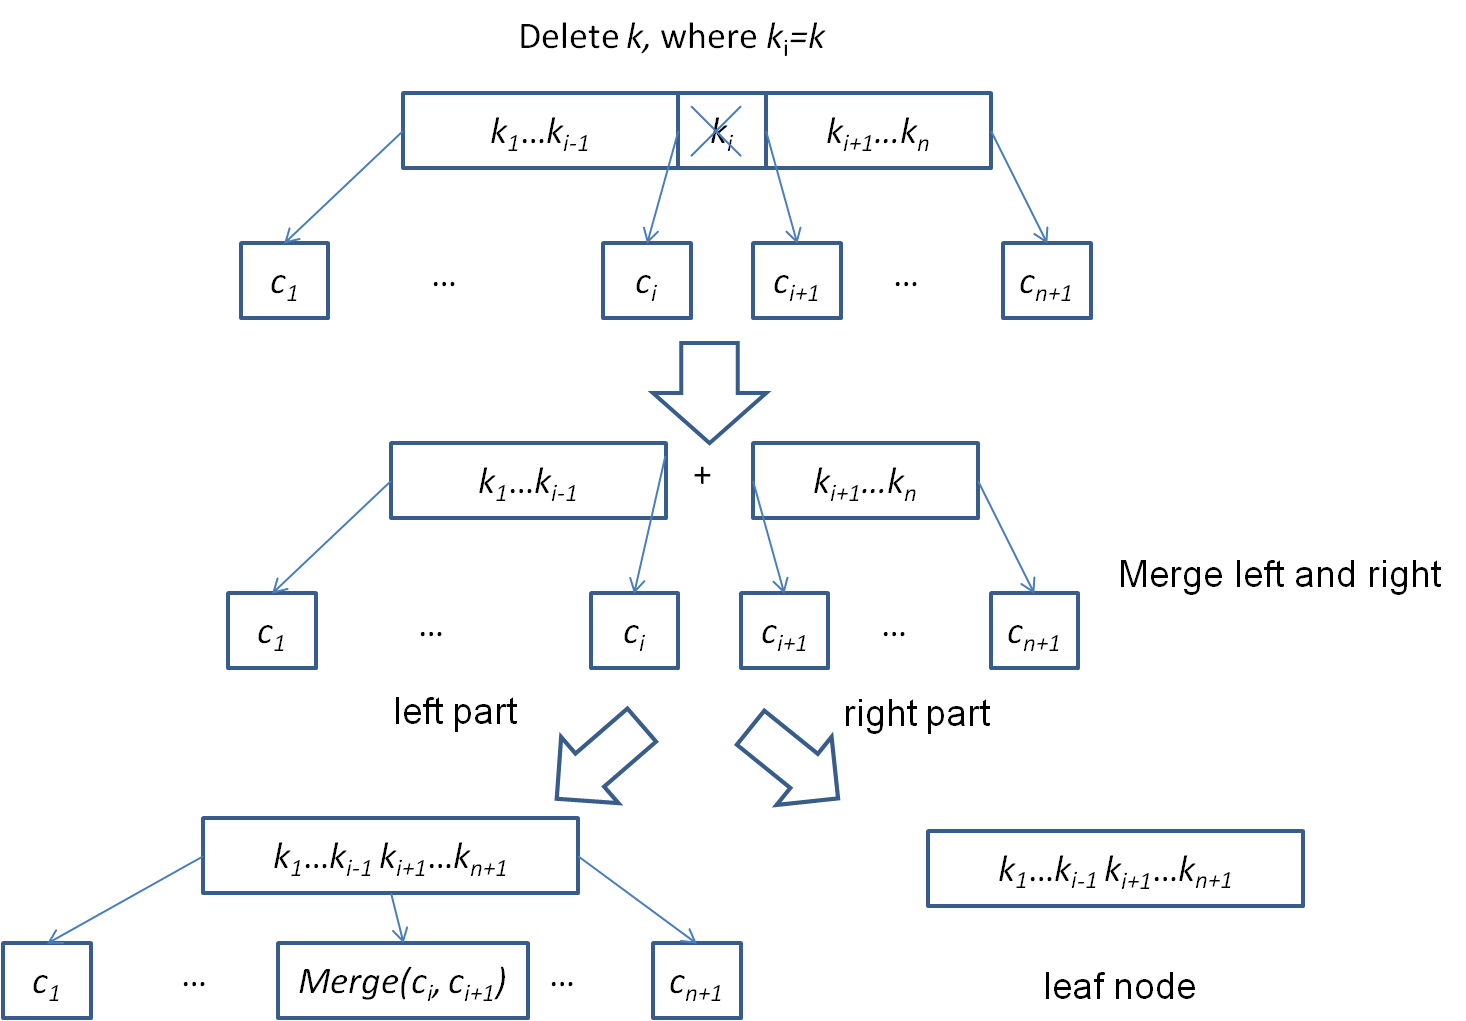
\includegraphics[scale=0.5]{img/btree-del-fp-merge.eps}
      \caption{Delete a key from a branch node. Removing $k_i$ breaks
the node into 2 parts, left part and right part. Merging these 2 parts
is a recursive process. When the two parts are leaves, the merging
terminates.} \label{fig:del-fp-merge}
    \end{center}
\end{figure}

When do merging, if the two nodes are not leaves, we merge the keys
together, and recursively merge the last child of the left part
and the first child of the right part as one new child node. Otherwise,
if they are leaves, we merely put all keys together.

Till now, we do the deleting in straightforward way. However, deleting
will decrease the number of keys of a node, and it may result in
violating the B-tree balance properties. The solution is to perform a
fixing along the path we traversed from root.

\begin{figure}[htbp]
    \begin{center}
      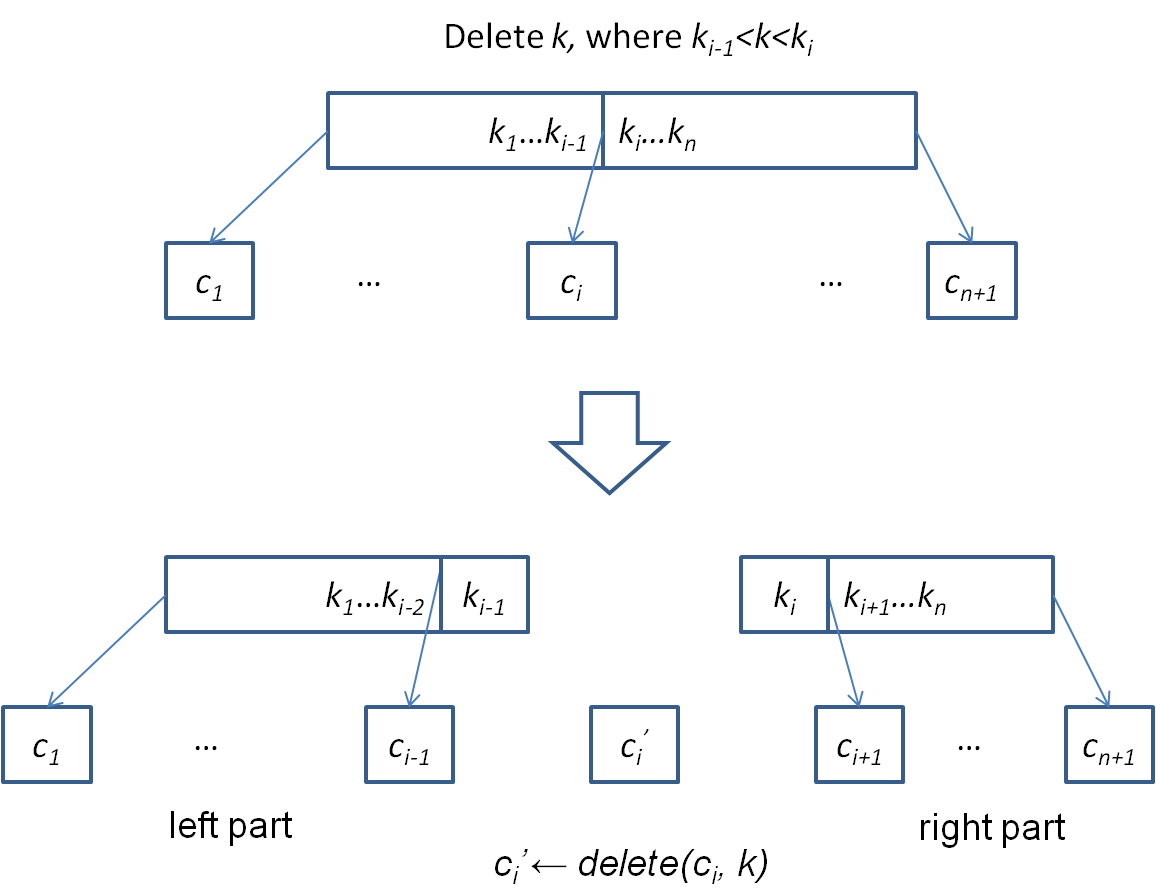
\includegraphics[scale=0.5]{img/btree-del-fp-make.eps}
      \caption{Denote $c_i'$ as the result of recursively deleting
key $k$, from child $c_i$, we should do fixing when making the
left part, $c_i'$ and right part together to a new node.} \label{fig:del-fp-make}
    \end{center}
\end{figure}

When we do recursive deletion, the branch node is broken into 3 parts.
The left part contains all keys less than $k$, say $k_1, k_2, ..., k_{i-1}$,
and children $c_1, c_2, ..., c_{i-1}$, the right part contains all keys
greater than $k$, say $k_i, k_{i+1}, ..., k_{n+1}$, and children
$c_{i+1}, c_{i+2}, ..., c_{n+1}$, the child $c_i$ which recursive deleting
applied becomes $c_i'$. We need make these 3 parts to a new node
as shown in figure \ref{fig:del-fp-make}.

At this time point, we can examine if $c_i'$ contains enough keys,
it the number of keys is to less (less than $t-1$, but not $t$ in
contrast to merge and delete approach), we can either borrow a key-child
pair from left part or right part, and do a inverse operation of
splitting. Figure \ref{fig:del-fp-fixlow} shows an example of borrow from left part.

\begin{figure}[htbp]
    \begin{center}
      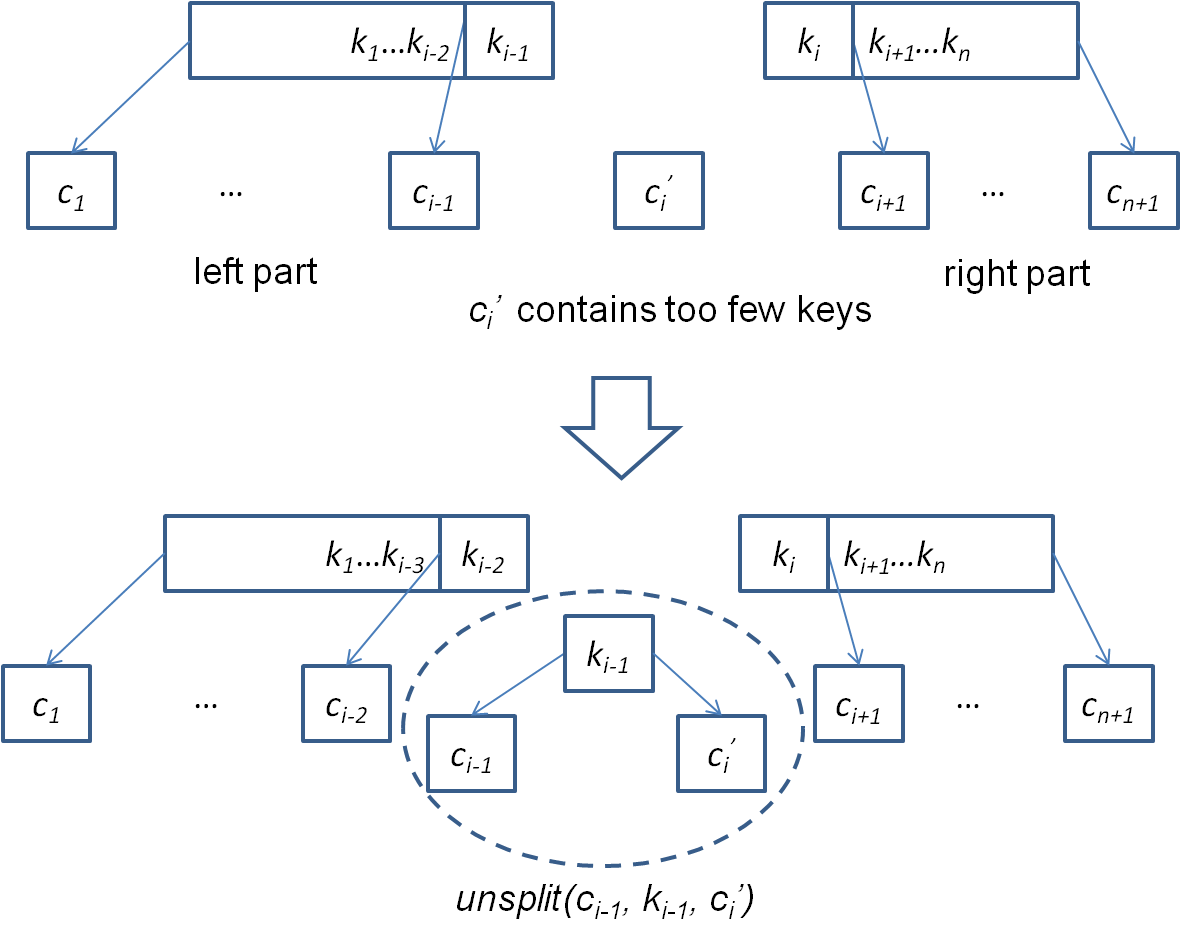
\includegraphics[scale=0.5]{img/btree-del-fp-fixlow.eps}
      \caption{Borrow a key-child pair from left part and
un-split to a new child.} \label{fig:del-fp-fixlow}
    \end{center}
\end{figure}

In case both left part and right part is empty, we can simply
push $c_i'$ up.

\subsubsection{Delete and fix algorithm implemented functionally}

By summarize all above analysis, we can draft the delete and fix
algorithm.

\begin{algorithmic}[1]
\Function{B-TREE-DELETE'}{$T, k$}
  \State \Return $FIX-ROOT(DEL(T, k))$
\EndFunction

\Function{DEL}{$T, k$}
  \If{$CHILDREN(T) = NIL$}\Comment{leaf node}
    \State $DELETE(KEYS(T), k)$
    \State \Return $T$
  \Else \Comment{branch node}
    \State $n \gets LENGTH(KEYS(T))$
    \State $i \gets LOWER-BOUND(KEYS(T), k)$
    \If{$KEYS(T)[i] = k$}
      \State $k_l \gets KEYS(T)[1, ..., i-1]$
      \State $k_r \gets KEYS(T)[i+1, ..., n]$
      \State $c_l \gets CHILDREN(T)[1, ..., i]$
      \State $c_r \gets CHILDREN(T)[i+1, ..., n+1]$
      \State \Return $MERGE(CREATE-B-TREE(k_l, c_l), CREATE-B-TREE(k_r, c_r))$
    \Else
      \State $k_l \gets KEYS(T)[1, ..., i-1]$
      \State $k_r \gets KEYS(T)[i, ..., n]$
      \State $c \gets CHILDREN(T)[i]$
      \State $c_l \gets CHILDREN(T)[1, ..., i-1]$
      \State $c_r \gets CHILDREN(T)[i+1, ..., n+1]$
      \State \Return $MAKE((k_l, c_l), c, (k_r, c_r))$
    \EndIf
  \EndIf
\EndFunction
\end{algorithmic}

The main delete function will call an internal $DEL$ function to
performs the work, after that, it will apply $FIX-ROOT$ to check
if need to shrink the tree height. So the $FIX-ROOT$ function we
defined in insertion section should be updated as the following.

\begin{algorithmic}[1]
\Function{FIX-ROOT}{$T$}
  \If{$KEYS(T) = NIL$} \Comment{Single child, shrink the height}
    \State $T \gets CHILDREN(T)[1]$
  \ElsIf{$FULL?(T)$}
    \State $T \gets B-TREE-SPLIT(T)$
  \EndIf
  \State \Return $T$
\EndFunction
\end{algorithmic}

For the recursive merging, the algorithm is given as below.
The left part and right part are passed as parameters. If
they are leaves, we just put all keys together. Otherwise,
we recursively merge the last child of left and the first child
of right to a new child, and make this new merged child and
the other two parts it breaks into a new node.

\begin{algorithmic}[1]
\Function{MERGE}{$L, R$}
  \If{$L, R$ are leaves}
    \State $T \gets CREATE-NEW-NODE()$
    \State $KEYS(T) \gets KEYS(L)+KEYS(R)$
    \State \Return $T$
  \Else
    \State $m gets LENGTH(KEYS(L))$
    \State $n gets LENGTH(KEYS(R))$
    \State $k_l \gets KEYS(L)$
    \State $k_r \gets KEYS(R)$
    \State $c_l \gets CHILDREN(L)[1, ..., m-1]$
    \State $c_r \gets CHILDREN(R)[2, ..., n]$
    \State $c \gets MERGE(CHILDREN(L)[m], CHILDREN(R)[1])$
    \State \Return $MAKE-B-TREE((k_l, c_l), c, (k_r, c_r))$
  \EndIf
\EndFunction
\end{algorithmic}

In order to make the three parts, the left $L$, the right $R$ and
the child $c_i'$ into a node, we need examine if $c_i$ contains
enough keys, together with the process of ensure it contains not too
much keys during insertion, we updated the algorithm like the following.

\begin{algorithmic}[1]
\Function{MAKE-B-TREE}{$L, C, R$}
  \If{$FULL?(C)$}
    \State \Return $FIX-FULL(L, C, R)$
  \ElsIf{$LOW?(C)$}
    \State \Return $FIX-LOW(L, C, R)$
  \Else
    \State $T \leftarrow CREATE-NEW-NODE()$
    \State $KEYS(T) \leftarrow KEYS(L) + KEYS(R)$
    \State $CHILDREN(T) \leftarrow CHILDREN(L)+[C]+CHILDREN(R)$
    \State \Return $T$
  \EndIf
\EndFunction
\end{algorithmic}

Where $FIX-LOW$ is defined as the following. In case the left part
isn't empty, it will borrow a key-child pair from the left, and
do un-split to make the child contains enough keys, then recursively
call $MAKE-B-TREE$; If the left part is empty, it will try to borrow
key-child pair from the right part, and if both sides are empty, it
will returns the child node as result, so that the height shrinks.

\begin{algorithmic}[1]
\Function{FIX-LOW}{$L, C, R$}
  \State $k_l, c_l \gets L$
  \State $k_r, c_r \gets R$
  \State $m \gets LENGTH(k_l)$
  \State $n \gets LENGTH(k_r)$
  \If{$k_l \ne NIL$}
    \State $k_l' \gets k_l[1, ..., m-1]$
    \State $c_l' \gets c_l[1, ..., m-1]$
    \State $C' \gets UN-SPLIT(c_l[m], k_l[m], C)$
    \State \Return $MAKE-B-TREE((k_l', c_l'), C', R)$
  \ElsIf{$k_r \ne NIL$}
    \State $k_r' \gets k_r[2, ..., n]$
    \State $c_r' \gets c_r[2, ..., n]$
    \State $C' \gets UN-SPLIT(C, k_r[1], c_r[1])$
    \State \Return $MAKE-B-TREE(L, C', (k_r', c_r'))$
  \Else
    \State \Return $C$
  \EndIf
\EndFunction
\end{algorithmic}

Function $UN-SPLIT$ defines as the inverses operation of splitting.

\begin{algorithmic}[1]
\Function{UN-SPLIT}{$L, k, R$}
  \State $T \gets CREATE-B-TREE-NODE()$
  \State $KEYS(T) \gets KEYS(L)+[k]+KEYS(R)$
  \State $CHILDREN(T) \gets CHILDREN(L)+CHILDREN(R)$
  \State \Return $T$
\EndFunction
\end{algorithmic}

\subsubsection{Delete and fix algorithm implemented in Haskell}
Based on the analysis of delete-then-fixing approach, a Haskell
program can be provided accordingly.

The core deleting function is simple, it just call an internal
removing function, then examine the root node to see if the
height of the tree can be shrunk.

\lstset{language=Haskell}
\begin{lstlisting}
import qualified Data.List as L

delete :: (Ord a) => BTree a -> a -> BTree a
delete tr x = fixRoot $ del tr x

del:: (Ord a) => BTree a -> a -> BTree a
del (Node ks [] t) x = Node (L.delete x ks) [] t
del (Node ks cs t) x =
    case L.elemIndex x ks of
      Just i -> merge (Node (take i ks) (take (i+1) cs) t)
                      (Node (drop (i+1) ks) (drop (i+1) cs) t)
      Nothing -> make (ks', cs') (del c x) (ks'', cs'')
    where
      (ks', ks'') = L.partition (<x) ks
      (cs', (c:cs'')) = L.splitAt (length ks') cs
\end{lstlisting} %$

Let's focus on the `del' function, if try to delete a key from
a leaf node, it just calls delete function defined in Data.List
library. If the key doesn't exist at all, the pre-defined
delete function will simply return the list without any modification.
For the case of deleting a key from a branch node, it will first examine
if the key can be located in this node, and apply recursive merge
after remove this key. Otherwise, it will locate the proper child
and do recursive delete-then-fixing on this child.

Note that `partition' and 'splitAt' functions defined in Data.List
can help to split the key and children list at the position that
all elements on the left is less than the key while the right part
are greater than the key.

The recursive merge program has two patterns, merge two leaves and
merge two branches. It is given as the following.

\begin{lstlisting}
merge :: BTree a -> BTree a -> BTree a
merge (Node ks [] t) (Node ks' [] _) = Node (ks++ks') [] t
merge (Node ks cs t) (Node ks' cs' _) = make (ks, init cs)
                                             (merge (last cs) (head cs'))
                                             (ks', tail cs')
\end{lstlisting}

Where `init', `last', 'tail' functions are used to manipulate
list which are defined in Haskell prelude.

The fixing part of delete-then-fixing is defined inside 'make'
function.

\begin{lstlisting}
make :: ([a], [BTree a]) -> BTree a -> ([a], [BTree a]) -> BTree a
make (ks', cs') c (ks'', cs'')
    | full c = fixFull (ks', cs') c (ks'', cs'')
    | low c  = fixLow  (ks', cs') c (ks'', cs'')
    | otherwise = Node (ks'++ks'') (cs'++[c]++cs'') (degree c)
\end{lstlisting}

Where function `low' is used to test if a node contains too few keys.

\begin{lstlisting}
low::BTree a -> Bool
low tr = (length $ keys tr) < (degree tr)-1
\end{lstlisting} %$

The real fixing is implemented by try to borrow keys either from
left sibling or right sibling as the following.

\begin{lstlisting}
fixLow :: ([a], [BTree a]) -> BTree a -> ([a], [BTree a]) -> BTree a
fixLow (ks'@(_:_), cs') c (ks'', cs'') = make (init ks', init cs')
                                              (unsplit (last cs') (last ks') c)
                                              (ks'', cs'')
fixLow (ks', cs') c (ks''@(_:_), cs'') = make (ks', cs')
                                              (unsplit c (head ks'') (head cs''))
                                              (tail ks'', tail cs'')
fixLow _ c _ = c
\end{lstlisting}

Note that by using `x@(\_:\_)' like pattern can help to ensure 'x' is
not empty. Here function `unsplit' is used which will do inverse
splitting operation like below.

\begin{lstlisting}
unsplit :: BTree a -> a -> BTree a -> BTree a
unsplit c1 k c2 = Node ((keys c1)++[k]++(keys c2))
                       ((children c1)++(children c2)) (degree c1)
\end{lstlisting}

In order to verify the Haskell program, we can provide some simple
test cases.

\begin{lstlisting}
import Control.Monad (foldM_, mapM_)

testDelete = foldM_ delShow (listToBTree "GMPXACDEJKNORSTUVYZBFHIQW" 3) "EGAMU"
  where
    delShow tr x = do
      let tr' = delete tr x
      putStrLn $ "delete "++(show x)
      putStrLn $ toString tr'
      return tr'
\end{lstlisting}

Where function `listToBTree' and `toString' are defined in previous section when we
explain insertion algorithm.

Run this function will generate the following result.

\begin{verbatim}
delete 'E'
((('A', 'B'), 'C', ('D', 'F'), 'G', ('H', 'I', 'J', 'K')), 'M',
(('N', 'O'), 'P', ('Q', 'R', 'S'), 'T', ('U', 'V'), 'W', ('X', 'Y', 'Z')))
delete 'G'
((('A', 'B'), 'C', ('D', 'F'), 'H', ('I', 'J', 'K')), 'M',
(('N', 'O'), 'P', ('Q', 'R', 'S'), 'T', ('U', 'V'), 'W', ('X', 'Y', 'Z')))
delete 'A'
(('B', 'C', 'D', 'F'), 'H', ('I', 'J', 'K'), 'M', ('N', 'O'),
'P', ('Q', 'R', 'S'), 'T', ('U', 'V'), 'W', ('X', 'Y', 'Z'))
delete 'M'
(('B', 'C', 'D', 'F'), 'H', ('I', 'J', 'K', 'N', 'O'), 'P',
('Q', 'R', 'S'), 'T', ('U', 'V'), 'W', ('X', 'Y', 'Z'))
delete 'U'
(('B', 'C', 'D', 'F'), 'H', ('I', 'J', 'K', 'N', 'O'), 'P',
('Q', 'R', 'S', 'T', 'V'), 'W', ('X', 'Y', 'Z'))
\end{verbatim}

If we try to delete the same key from the same B-tree as in merge and fixing
approach, we can found that the result is different by using delete-then-fixing
methods. Although the results are not as same as each other, both satisfy
the B-tree properties, so they are all correct.

\begin{figure}[htbp]
    \begin{center}
      \includegraphics[scale=0.5]{img/btree-del-fp-before.ps}

      a. A B-tree before performing deleting;

      \includegraphics[scale=0.5]{img/btree-del-fp-E.ps}

      b. After delete key 'E'
      \caption{Result of delete-then-fixing (1)} \label{fig:result-del-fp1}
    \end{center}
\end{figure}

\begin{figure}[htbp]
    \begin{center}
      \includegraphics[scale=0.5]{img/btree-del-fp-G.ps}

      c. After delete key 'G';

      \includegraphics[scale=0.5]{img/btree-del-fp-A.ps}

      d. After delete key 'A';
      \caption{Result of delete-then-fixing (2)} \label{fig:result-del-fp2}
    \end{center}
\end{figure}

\begin{figure}[htbp]
    \begin{center}
      \includegraphics[scale=0.5]{img/btree-del-fp-M.ps}

      e. After delete key 'M';

      \includegraphics[scale=0.5]{img/btree-del-fp-U.ps}

      f. After delete key 'U';
      \caption{Result of delete-then-fixing (3)} \label{fig:result-del-fp3}
    \end{center}
\end{figure}


\subsubsection{Delete and fix algorithm implemented in Scheme/Lisp}
In order to implement delete program in Scheme/Lisp, we provide an
extra function to test if a node contains too few keys after deletion.

\lstset{language=lisp}
\begin{lstlisting}
(define (low? tr t) ;; t: minimum degree
  (< (length (keys tr))
     (- t 1)))
\end{lstlisting}

And some general purpose list manipulation functions are defined.

\begin{lstlisting}
(define (rest lst k)
  (list-tail lst (- (length lst) k)))

(define (except-rest lst k)
  (list-head lst (- (length lst) k)))

(define (first lst)
  (if (null? lst) '() (car lst)))

(define (last lst)
  (if (null? lst) '() (car (last-pair lst))))

(define (inits lst)
  (if (null? lst) '() (except-last-pair lst)))
\end{lstlisting}

Function `rest' can extract the last $k$ elements from a list, while
`except-rest' used to extract all except the last $k$ elements.
`first' can be treat as a safe `car', it will return empty list but not
throw exception when the list is empty. Function `last' returns the
last element of a list, and if the list is empty, it will return
empty result. Function `inits' returns all excluding the last element.

And a inversion operation of splitting is provided.

\begin{lstlisting}
(define (un-split lst)
  (let ((c1 (car lst))
	(k (cadr lst))
	(c2 (caddr lst)))
    (append c1 (list k) c2)))
\end{lstlising}

The main function of deletion is defined as the following.

\begin{lstlisting}
(define (btree-delete tr x t)
  (define (del tr x)
    (if (leaf? tr)
	(delete x tr)
	(let* ((res (partition-by tr x))
	       (left (car res))
	       (c (cadr res))
	       (right (caddr res)))
	  (if (equal? (first right) x)
	      (merge-btree (append left (list c)) (cdr right) t)
	      (make-btree left (del c x) right t)))))
  (fix-root (del tr x) t))
\end{lstlisting}

It is implemented in a similar way as the insertion, call an internal
defined `del' function then apply fixing process on it. In the internal
deletion fiction, if the B-tree is a leaf node, the standard list
deleting function defined in standard library is applied. If it is
a branch node, we call the `partition-by' function defined previously.
This function will divide the node into 3 parts, all children and
keys less than $x$ as the left part, a child node next, all keys not less
than (greater than or equal to) $x$ and children s the right part.

If the first key in right part is equal to $x$, it means $x$ can
be located in this node, we remove $x$ from right and then
call `merge-btree' to merge left+c, right-$x$ to one new node.

\begin{lstlisting}
(define (merge-btree tr1 tr2 t)
  (if (leaf? tr1)
      (append tr1 tr2)
      (make-btree (inits tr1)
		  (merge-btree (last tr1) (car tr2) t)
		  (cdr tr2)
		  t)))
\end{lstlisting}

Otherwise, $x$ may be located in c, so we need recursively try
to delete $x$ from c.

Function `fix-root' is updated to handle the cases for deletion
as below.

\begin{lstlisting}
(define (fix-root tr t)
  (cond ((null? tr) '()) ;; empty tree
	((full? tr t) (split tr t))
	((null? (keys tr)) (car tr)) ;; shrink height
	(else tr)))
\end{lstlisting}

We added one case to handle if a node contains too few keys
after deleting in `make-btree'.

\begin{lstlisting}
(define (make-btree l c r t)
  (cond ((full? c t) (fix-full l c r t))
	((low? c t) (fix-low l c r t))
	(else (append l (cons c r)))))
\end{lstlisting}

Where `fix-low' is defined to try to borrow a key and a child
either from left sibling or right sibling.

\begin{lstlisting}
(define (fix-low l c r t)
  (cond ((not (null? (keys l)))
	 (make-btree (except-rest l 2)
		     (un-split (append (rest l 2) (list c)))
		     r t))
	((not (null? (keys r)))
	 (make-btree l
		     (un-split (cons c (list-head r 2)))
		     (list-tail r 2) t))
	(else c)))
\end{lstlisting}

In order to verify the the deleting program, a simple test is
fed to the above defined function.

\begin{lstlisting}
(define (test-delete)
  (define (del-and-show tr x)
    (let ((r (btree-delete tr x 3)))
      (begin (display r) (display "\n") r)))
  (fold-left del-and-show
	     (list->btree (str->slist "GMPXACDEJKNORSTUVYZBFHIQW") 3)
	     (str->slist "EGAMU")))
\end{lstlisting}

Run the test will generate the following result.

\begin{lstlisting}
(((A B) C (D F) G (H I J K)) M ((N O) P (Q R S) T (U V) W (X Y Z)))
(((A B) C (D F) H (I J K)) M ((N O) P (Q R S) T (U V) W (X Y Z)))
((B C D F) H (I J K) M (N O) P (Q R S) T (U V) W (X Y Z))
((B C D F) H (I J K N O) P (Q R S) T (U V) W (X Y Z))
((B C D F) H (I J K N O) P (Q R S T V) W (X Y Z))
\end{lstlisting}

Compare with the output by the Haskell program in previous section,
it can be found they are same.

% ================================================================
%               Searching
% ================================================================
\section{Searching}

Although searching in B-tree can be considered as a generalized
form of tree search which extended from binary search tree, it's good
to mention that in disk access case, instead of just returning the
satellite data corresponding to the key, it's more meaningful to
return the whole node, which contains the key.

\subsection{Imperative search algorithm}

When searching in Binary tree, there are only 2 different directions,
left and right to go further searching, however, in B-tree, we need
extend the search directions to cover the number of children in a
node.

\begin{algorithmic}[1]
\Function{B-TREE-SEARCH}{$T, k$}
  \Loop
    \State $i \gets 1$
    \While{$i \leq LENGTH(KEYS(T))$ and $k > KEYS(T)[i]$}
      \State $k \gets k+1$
    \EndWhile
    \If{$i \leq LENGTH(KEYS(T))$ and $k = KEYS(T)[i]$}
      \State \Return $(T, i)$
    \EndIf
    \If{$T$ is leaf}
      \State \Return $NIL$ \Comment{$k$ doesn't exist at all}
    \Else
      \State $T \gets CHILDREN(T)[i]$
    \EndIf
  \EndLoop
\EndFunction
\end{algorithmic}

When doing search, the program examine each key from the root node by
traverse from the smallest towards the biggest one. in case it find a
matched key, it returns the current node as well as the index of this
keys. Otherwise, if it finds this key satisfying $k_i < k < k_{i+1}$,
The program will update the current node to be examined as child node
$c_{i+1}$. If it
fails to find this key in a leaf node, empty value is returned to
indicate the fail case.

Note that in ``Introduction to Algorithm'', this program is described
with recursion, Here the recursion is eliminated.

\subsubsection*{search program in C++}
In C++ implementation, we can use pair provided in STL library as
the return type.

\lstset{language=C++}
\begin{lstlisting}
template<class T>
std::pair<T*, unsigned int> search(T* t, typename T::key_type k){
  for(;;){
    unsigned int i(0);
    for(; i < t->keys.size() && k > t->keys[i]; ++i);
    if(i < t->keys.size() && k == t->keys[i])
      return std::make_pair(t, i);
    if(t->leaf())
      break;
    t = t->children[i];
  }
  return std::make_pair((T*)0, 0); //not found
}
\end{lstlisting}

And the test cases are given as below.

\begin{lstlisting}
  void test_search(){
    std::cout<<"test search...\n";
    const char* ss[] = {"G", "M", "P", "X", "A", "C", "D", "E", "J", "K", \
                        "N", "O", "R", "S", "T", "U", "V", "Y", "Z"};
    BTree<std::string, 3>* tr = list_to_btree(ss, ss+sizeof(ss)/sizeof(char*),
                                              new BTree<std::string, 3>);
    std::cout<<"\n"<<btree_to_str(tr)<<"\n";
    for(unsigned int i=0; i<sizeof(ss)/sizeof(char*); ++i)
      __test_search(tr, ss[i]);
    __test_search(tr, "W");
    delete tr;
  }

  template<class T>
  void __test_search(T* t, typename T::key_type k){
    std::pair<T*, unsigned int> res = search(t, k);
    if(res.first)
      std::cout<<"found "<<res.first->keys[res.second]<<"\n";
    else
      std::cout<<"not found "<<k<<"\n";
  }
\end{lstlisting}

Run `test\_search' function will generate the following result.

\begin{verbatim}
test search...
((A, C), D, (E, G, J, K), M, (N, O), P, (R, S), T, (U, V, X, Y, Z))
found G
found M
...
found Z
not found W
\end{verbatim}

Here the program can find all keys we inserted.

\subsubsection*{search program in Python}

Change a bit the above algorithm in Python gets the program corresponding
to the pseudo code mentioned in ``Introduction to Algorithm'' textbook.

\lstset{language=Python}
\begin{lstlisting}
def B_tree_search(tr, key):
    for i in range(len(tr.keys)):
        if key<= tr.keys[i]:
            break
    if key == tr.keys[i]:
        return (tr, i)
    if tr.leaf:
        return None
    else:
        if key>tr.keys[-1]:
            i=i+1
        #disk_read
        return B_tree_search(tr.children[i], key)
\end{lstlisting}

There is a minor modification from the original pseudo code.
We uses for-loop to iterate the keys, the the boundary check is done
by compare the last key in the node and adjust the index if
necessary.

Let's feed some simple test cases to this program.

\begin{lstlisting}
   def test_search():
        lst = ["G", "M", "P", "X", "A", "C", "D", "E", "J", "K", \
               "N", "O", "R", "S", "T", "U", "V", "Y", "Z"]
        tr = list_to_B_tree(lst, 3)
        print "test search\n", B_tree_to_str(tr)
        for i in lst:
            __test_search__(tr, i)
        __test_search__(tr, "W")

    def __test_search__(tr, k):
        res = B_tree_search(tr, k)
        if res is None:
            print k, "not found"
        else:
            (node, i) = res
            print "found", node.keys[i]
\end{lstlisting}

Run the function `test\_search' will generate the following result.

\begin{verbatim}
found G
found M
...
found Z
W not found
\end{verbatim}

\subsection{Functional search algorithm}
The imperative algorithm can be turned into Functional by performing
recursive search on a child in case key can't be located in current
node.

\begin{algorithmic}[1]
\Function{B-TREE-SEARCH}{$T, k$}
  \State $i \gets FIND-FIRST( \lambda_xx>=k, KEYS(T))$
  \If{$i$ exists and $k = KEYS(T)[i]$}
    \State \Return $(T, i)$
  \EndIf
  \If{$T$ is leaf}
    \State \Return $NIL$ \Comment{$k$ doesn't exist at all}
  \Else
    \State \Return $B-TREE-SEARCH(CHILDREN(T)[i], k)$
  \EndIf
\EndFunction
\end{algorithmic}

\subsubsection*{Search program in Haskell}
In Haskell program, we first filter out all keys less than the
key to be searched. Then check the first element in the result.
If it matches, we return the current node along with the index
as a tuple. Where the index start from `0'. If it doesn't match,
We then do recursive search till leaf node.

\lstset{language=C++}
\begin{lstlisting}
search :: (Ord a)=> BTree a -> a -> Maybe (BTree a, Int)
search tr@(Node ks cs _) k
    | matchFirst k $ drop len ks = Just (tr, len)
    | otherwise = if null cs then Nothing
                  else search (cs !! len) k
    where
      matchFirst x (y:_) = x==y
      matchFirst x _ = False
      len = length $ filter (<k) ks
\end{lstlisting}

The verification test cases are provided as the following.

\begin{lstlisting}
testSearch = mapM_ (showSearch (listToBTree lst 3)) $ lst++"L"
    where
      showSearch tr x = do
        case search tr x of
          Just (_, i) -> putStrLn $ "found" ++ (show x)
          Nothing -> putStrLn $ "not found" ++ (show x)
      lst = "GMPXACDEJKNORSTUVYZBFHIQW"
\end{lstlisting} %$

Here we construct a B-tree from a series of string, then
we check if each element in this string can be located.
Finally, an non-existed element ``L'' is fed to verify the
failure case.

Run this test function generates the following results.

\begin{verbatim}
found'G'
found'M'
...
found'W'
not found'L'
\end{verbatim}

\subsubsection*{Search program in Scheme/Lisp}
Because we intersperse children and keys in one list in
Scheme/Lisp B-tree definition, the search function just
move one step a head to locate the key in a node.

\lstset{language=lisp}
\begin{lstlisting}
(define (btree-search tr x)
  ;; find the smallest index where keys[i]>= x
  (define (find-index tr x)
    (let ((pred (if (string? x) string>=? >=)))
      (if (null? tr)
	  0
	  (if (and (not (list? (car tr))) (pred (car tr) x))
	      0
	      (+ 1 (find-index (cdr tr) x))))))
  (let ((i (find-index tr x)))
    (if (and (< i (length tr)) (equal? x (list-ref tr i)))
	(cons tr i)
	(if (leaf? tr) #f (btree-search (list-ref tr (- i 1)) x)))))
\end{lstlisting}

The program defines an inner function to find the index of the
first element which is greater or equal to the key we are searching.

If the key pointed by this index matches, we are done. Otherwise,
this index points to a child which may contains this key. The program
will return false result in case the current node is a leaf node.

We can run the below testing function to verify this searching
program.

\begin{lstlisting}
(define (test-search)
  (define (search-and-show tr x)
    (if (btree-search tr x)
	(display (list "found " x))
	(display (list "not found " x))))
  (let* ((lst (str->slist "GMPXACDEJKNORSTUVYZBFHIQW"))
	 (tr (list->btree lst 3)))
    (map (lambda (x) (search-and-show tr x)) (cons "L" lst))))
\end{lstlisitng}

A non-existed key ``L'' is firstly fed, and then all elements
which used to form the B-tree are looked up for verification.

\begin{lstlisting}
(not found  L)(found  G)(found  M) ... (found  W)
\end{lstlisting}

% ================================================================
%                 Short summary
% ================================================================
\section{Notes and short summary}
In this post, we explained the B-tree data structure as a kind of
extension from binary search tree. The background knowledge of
magnetic disk access is skipped, user can refer to \cite{CLRS}
for detail. For the three main operations, insertion, deletion,
and searching, both imperative and functional algorithms are
illustrated. The complexity isn't discussed here, However, since
B-tree are defined to maintain the balance properties, all operations
mentioned here perform $O(lgN)$ where $N$ is the number of the
keys in a B-tree.

\begin{Exercise}
\begin{itemize}
\item Eleminate the recursion in imperative B-tree insertion algorithm.
\end{itemize}
\end{Exercise}
% ================================================================
%                 Appendix
% ================================================================
\section{Appendix} \label{appendix}
%\appendix
All programs provided along with this article are free for
downloading.

\subsection{Prerequisite software}
GNU Make is used for easy build some of the program. For C++ and ANSI C programs,
GNU GCC and G++ 3.4.4 are used.
For Haskell programs GHC 6.10.4 is used
for building. For Python programs, Python 2.5 is used for testing, for
Scheme/Lisp program, MIT Scheme 14.9 is used.

all source files are put in one folder. Invoke 'make' or 'make all'
will build C++ and Haskell program.

Run 'make Haskell' will separate build Haskell program. the executable
file is ``htest'' (with .exe
in Window like OS). It is also possible to run the program in GHCi.

\subsection{Tools}

Besides them, I use graphviz to draw most of the figures in this post. In order to
translate the B-tree output to dot script. A Haskell tool is provided.
It can be used like this.

\begin{verbatim}
bt2dot filename.dot "string"
\end{verbatim}

Where filename.dot is the output file for the dot script. It can
parse the string which describes B-tree content and translate it
into dot script.

This source code of this tool is BTr2dot.hs, it can also be downloaded
with this article.

download position: http://sites.google.com/site/algoxy/btree/btree.zip

\begin{thebibliography}{99}

\bibitem{CLRS}
Thomas H. Cormen, Charles E. Leiserson, Ronald L. Rivest and Clifford Stein. ``Introduction to Algorithms, Second Edition''. The MIT Press, 2001. ISBN: 0262032937.

\bibitem{wiki-b-tree}
B-tree, Wikipedia. http://en.wikipedia.org/wiki/B-tree

\bibitem{lxy-bst}
Liu Xinyu. ``Comparison of imperative and functional implementation of
binary search tree''. http://sites.google.com/site/algoxy/bstree

\bibitem{okasaki-rbtree}
Chris Okasaki. ``FUNCTIONAL PEARLS Red-Black Trees in a Functional Setting''. J. Functional Programming. 1998

\end{thebibliography}

\ifx\wholebook\relax \else
\end{document}
\fi
